\documentclass[ngerman, a4paper, justified, nobib, notoc, sfsidenotes]{tufte-book}
\usepackage[ngerman]{babel}
\usepackage{mathtools}
\usepackage{amsfonts, amssymb}
\usepackage{graphicx}
\usepackage{tikz}
\usepackage{algorithm}
\usepackage{algpseudocode}
\usepackage{varioref}
\usepackage{hyperref}
\usepackage{cleveref}
\usepackage{siunitx}
\usepackage{enumitem}
\usepackage{xcolor}
\usepackage[babel]{csquotes}
\usepackage{tikzsymbols}
\usepackage{float}
\usepackage{hhline}
\usepackage{longtable}
\usepackage{standalone}
\usepackage{pgfplots}
\usepackage[ngerman]{datetime2}
\usepackage[backend=biber, style=ieee]{biblatex}
\usepackage{tabularx}
\usepackage{fontspec}
\usepackage{caption}
\usepackage{tabu}
\usepackage{minted}
\usepackage{newfloat}
\usepackage{tocloft}
\DeclareFloatingEnvironment[name=Quelltext]{mylisting}

\setminted{
	fontsize=\small,
	tabsize=4,
	autogobble
}

\pgfplotsset{compat=1.18}

\usetikzlibrary{tikzlings}
\usetikzlibrary{patterns, positioning, shapes.geometric, shapes.callouts, arrows.meta, graphs}

\addbibresource{sources.bib}
\addbibresource{pictures.bib}

\makeatletter
\@twosidefalse
\@mparswitchfalse
\makeatother

\newfontfamily\garamondfont{EB Garamond}[Weight=200]
\newfontfamily\marginfont{LucidaSansOT}

\usepackage{fontspec}
\usepackage{microtype}
\usepackage{unicode-math}

\setmainfont{Lucida Bright OT}
\setmathfont{Lucida Bright Math OT}

\setlength{\parindent}{0pt}
\setlength{\RaggedRightParindent}{0pt}
\setlength{\JustifyingParindent}{0pt}
\setlength{\parskip}{1em}

\makeatletter
\renewcommand{\@tufte@marginfont}{\marginfont\scriptsize}
\renewcommand{\captionlabelfont}{\marginfont\color{gray}\scriptsize}
\renewcommand{\captionfont}{\marginfont\scriptsize}
\makeatother

\usepackage{sectsty}
\subsectionfont{\normalfont\large}
\sectionfont{\normalfont\Large\upshape}
\chaptertitlefont{\normalfont\LARGE}


\usepackage{titlesec}

\titleformat{\part}[display]
{\normalfont\huge} 
{\partname~\thepart} 
{20pt}
{\Huge}

\linespread{1.15}

\definecolor{gold}{rgb}{0.980, 0.706, 0.216}

\hypersetup{
	colorlinks=true,         
	linkcolor=gold,          
	urlcolor=blue,           
	citecolor=gold,           
	pdfborder={0 0 0},       
}

%lstlisting
\definecolor{main-color}{rgb}{0.6627, 0.7176, 0.7764}
\definecolor{back-color}{rgb}{0.94,0.94,0.94}
\definecolor{string-color}{rgb}{0.3333, 0.5254, 0.345}
\definecolor{key-color}{rgb}{0.13,0.13,1}
\definecolor{typedef-color}{rgb}{0.8, 0.47, 0.196}
\definecolor{func-red}{rgb}{1, 0.7, 0.56}

\setlength{\cftbeforesecskip}{5pt}
\setlength{\cftbeforechapskip}{10pt}
\renewcommand{\cftsecfont}{\normalfont}  
\renewcommand{\cftsecpagefont}{\normalfont}
\renewcommand{\cfttoctitlefont}{\LARGE\mdseries}

\numberwithin{figure}{part}
\numberwithin{table}{part}
\numberwithin{equation}{part}
\numberwithin{mylisting}{part}
\renewcommand{\thepart}{\arabic{part}}


\MakeOuterQuote{"}


\title{Turing-Welchman-Bombe}

\begin{document}
	
	\begin{fullwidth}
		\begin{center}
			\garamondfont
			\thispagestyle{empty}
			\vspace*{3cm}
			{\huge\scshape\textcolor{gray}{Turing-Welchman-Bombe\\}}
			\vspace{5cm}
			\large
			Projektarbeit zur Kryptoanalyse der Enigma-Maschine durch eine\\ 
			Software-Nachbildung der Turing-Welchman-Bombe\\
			der Fakultät Elektrotechnik und Informatik\\
			\vspace{2cm}
			\textit{von} Emanuel Schäffer 
			\hspace{0.4cm} \textcolor{gray}{\rule[-.2em]{0.6pt}{1.2em}} \hspace{0.4cm} 
			\DTMtoday\\
			\vspace{2cm}
			%	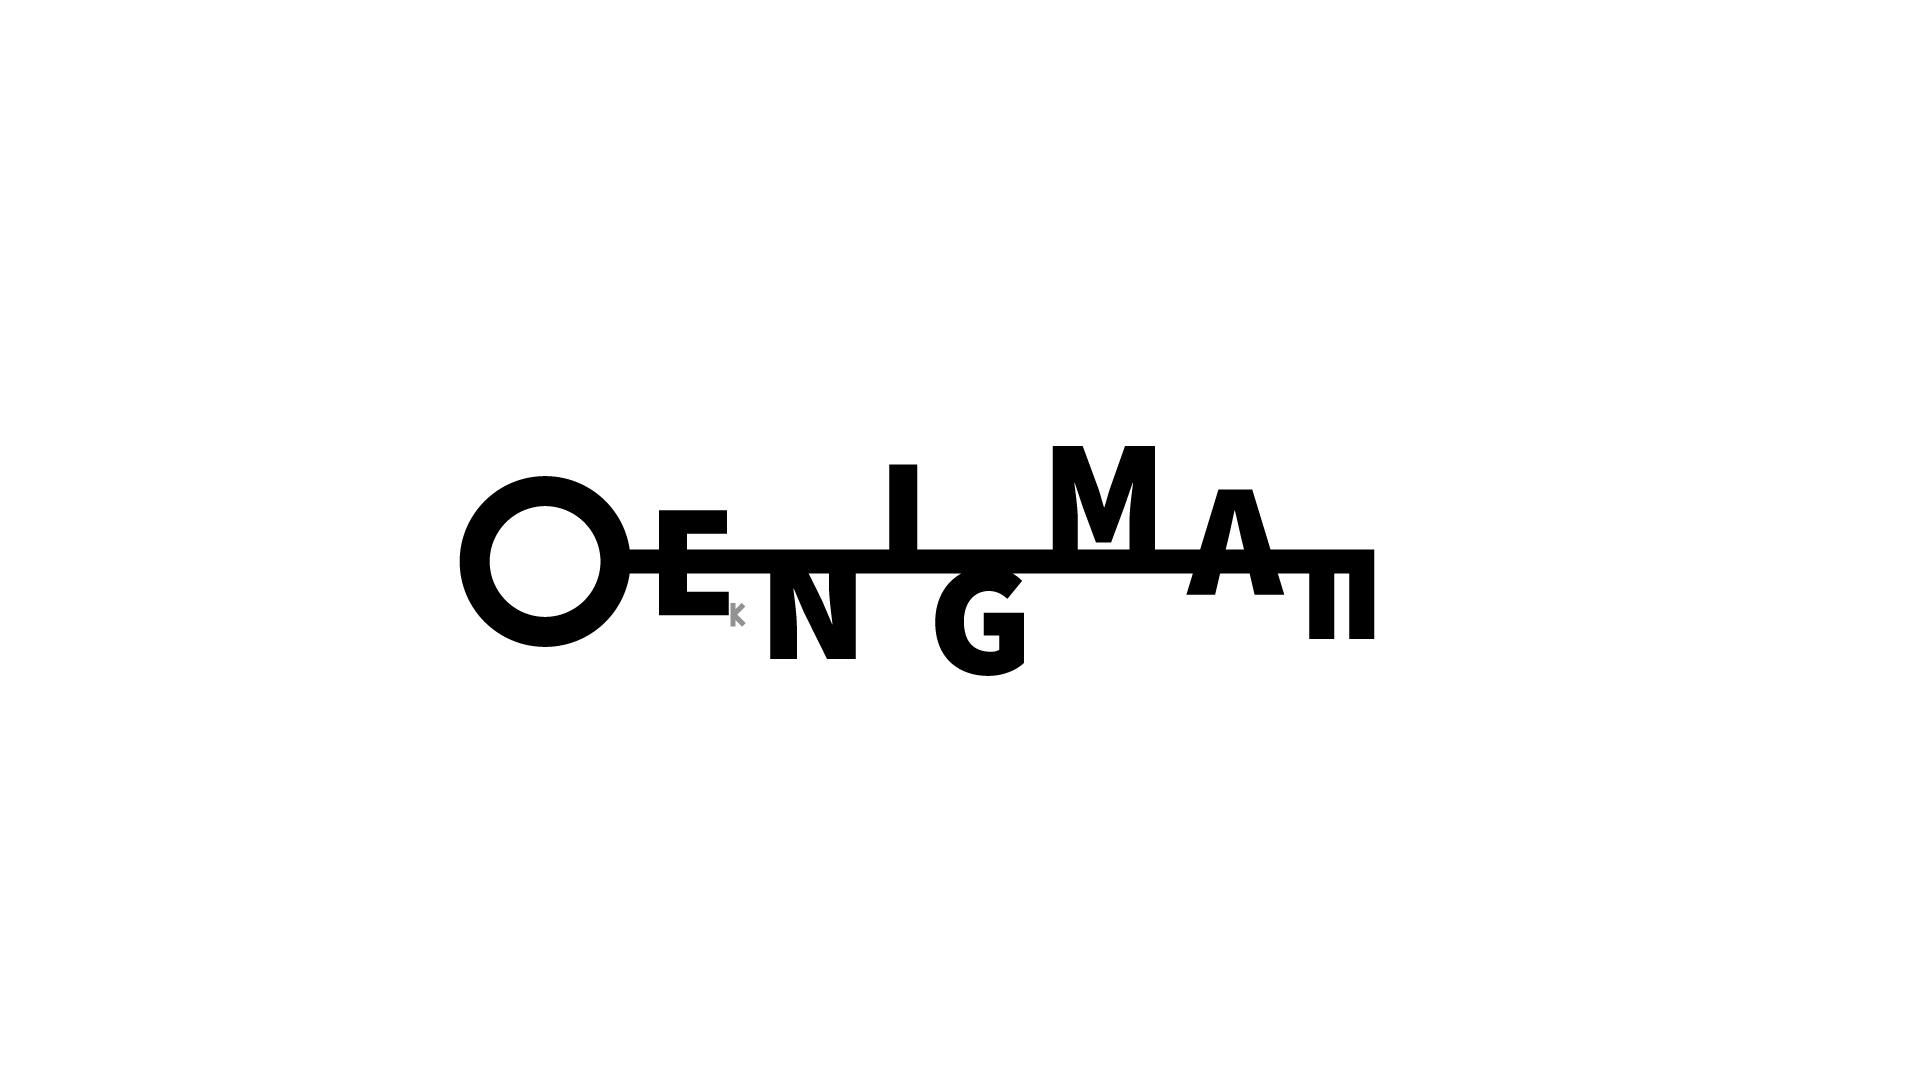
\includegraphics[width=.7\linewidth]{Logos-Enigma}
			\vfill
			\textsl{RWU--University of Applied Sciences\\Prof. Dipl.-Math. Ekkehard Löhmann}
			\normalsize
		\end{center}
	\end{fullwidth}
	
	\frontmatter
	\fontsize{8.5}{11.7}\selectfont

	\chapter*{\textit{Kolophon}}
	Dieses Dokument wurde mit \LaTeX{} gesetzt\\ und verwendet die \textsl{Lucida} Schriftart.
	
	\chapter*{\textit{Dankesworte}}
	Mein besonderer Dank gilt meinen Eltern, die mir durch Ihre Unterstützung und Ermutigung stets zur Seite stehen.
	
	Ein großes Dankeschön an Lea Rutzer und Paul Köster, die sich die Zeit genommen haben, meine Arbeit gegenzulesen.
	
	\clearpage
	\begin{fullwidth}
		\tableofcontents
	\end{fullwidth}
	
	\chapter*{Einleitung}\label{ch:einleitung}

	Diese Projektarbeit beschäftigt sich mit der Kryptoanalyse der Enigma-Maschine.
	Im Speziellen wird hier auf die Kryptoanalyse mit der von Alan Turing und Gordon Welchman entwickelten \glqq Turing-Welchman-Bombe\grqq{} eingegangen.
	Die Turing-Welchman-Bombe baut auf die Arbeit von Marian Rejewski und seiner \glqq Bomba\grqq{} auf, welche der Turing-Welchman-Bombe ihren Namen gab.
	Dieses Verfahren zur Kryptoanalyse spielte eine wesentliche Rolle im Zweiten Weltkrieg und trug nach der Meinung vieler Historiker maßgeblich dazu bei, den Krieg zu verkürzen und rettete somit zahlreiche Menschenleben.
	% 2 Jahre 14 Mio. Menschenleben
	
	\mainmatter
	
	%\chapter{Die}\label{ch:die-enigma}
\part{Die Enigma-Maschine}\label{ch:die-enigma}
\chapter{Einführung}\label{sec:einfuhrung}
Um die Funktionsweise der Turing-Welchman-Bombe und ihrer Software-Nach\-bil\-dung zu verstehen, muss zuerst die Enigma-Maschine verstanden werden.
Im Folgenden sei ein Überblick über die Enigma-Maschine gegeben.
Die Enigma-Ma\-schine ist eine Rotor-Chiffrier\-maschine, die 1918 von Arthur Scherbius zum Patent angemeldet wurde und hauptsächlich im Zweiten Weltkrieg zum Einsatz kam.
Aufgrund der Sicherheitsanforderungen der deutschen Wehrmacht wurde die kommerziell erwerbliche Enigma-Maschine modifiziert.
In \cref{fig:enigma_complete} ist eine solche modifizierte Enigma-Maschine zu sehen.
Die von der Wehrmacht eingesetzten Enigma-Maschinen verfügten zunächst über drei Walzen~(Ziffer~13).
Neuerungen waren das Steckerbrett~(siehe~\cref{fig:enigma_complete}~front) und gegen Ende des Krieges eine zusätzliche, vierte Walze. 
Adaptiert wurde die Umkehrwalze~(Ziffer~20).
Hier wird, wenn nicht ausdrücklich erwähnt, ausschließlich die Enigma M3 mit drei Walzen betrachtet.
\begin{figure}
	\centering
	\includegraphics[width=.6\linewidth]{Enigma/Enigma-plakat}
	\caption{Die Enigma-Maschine (Foto Deutsches Museum München)}
	\label{fig:enigma_complete}
\end{figure}

\chapter{Funktionsweise}\label{sec:funktionsweise}

\section{Walzen}\label{subsec:walzen}
Jede der von der Enigma-Maschine verwendeten Walzen besitzt eine interne Verdrahtung, welche eine monoalphabetische Substitution durchführt.
Das bedeutet, dass jeder Buchstabe auf genau einen anderen Buchstaben abgebildet wird.
In~\cref{fig:rot1_wiring} ist die Verdrahtung der Walze~I zu sehen.

\begin{figure}
	\centering
	\caption{Verdrahtung Walze I}
	\resizebox{\textwidth}{!}{%
		\begin{tabular}{|c|c|c|c|c|c|c|c|c|c|c|c|c|c|c|c|c|c|c|c|c|c|c|c|c|c|}
			\hline
			A & B & C & D & E & F & G & H & I & J & K & L & M & N & O & P & Q & R & S & T & U & V & W & X & Y & Z\\
			\hline
			E & K & M & F & L & G & D & Q & V & Z & N & T & O & W & Y & H & X & U & S & P & A & I & B & R & C & J\\
			\hline
		\end{tabular}
	}
	\label{fig:rot1_wiring}
\end{figure}

Diese Verdrahtung ist starr und individuell für jede Walze.
Eine Enigma-Walze hat 26 Eingangs- und 26 Ausgangs-Kontakte.
Zudem kann eine Walze 26 Ausgangspositionen annehmen, jeweils repräsentativ für das Alphabet.
Wird nun an den Eingangskontakt \glqq A\grqq{} Spannung angelegt, so wird dieser Buchstabe durch die interne Verdrahtung zu einem \glqq E\grqq{} permutiert.

Um die Enigma-Maschine in Betrieb zu nehmen, müssen drei von acht möglichen Walzen ausgewählt werden.
Diese drei Walzen werden in Reihe geschaltet.
Die rechte Walze wird bei jedem Tastendruck um eine Position weitergerückt.
Hat diese Walze eine komplette Rotation vollzogen, rückt die Walze links neben ihr um eine Position weiter.\footnote{Eine Analogie hierfür ist das Verhalten eines mechanischen Kilometerzählers oder das Verhalten von Sekunden-, Minuten- und Studenzeigern einer Uhr.}
Die 26 Eingangs-Kontakte der rechten Walze werden durch 26 Kontakte der Enigma-Maschine versorgt.
Diese sind mit der Tastatur verbunden.
Die Enigma-Maschinen Kontakte sind starr und bewegen sich nicht.
Wird nun ein \glqq A\grqq{} betätigt, während sich die Walze in Stellung \glqq A\grqq{} befindet, wird diese zuerst rotiert und dann durchlaufen.
Der Strom nimmt somit den \glqq B\grqq{} Pfad.
Das Resultat dieser in Reihe geschalteten Walzen ist eine polyalphabetische Substitution.

\begin{figure}
	\centering
	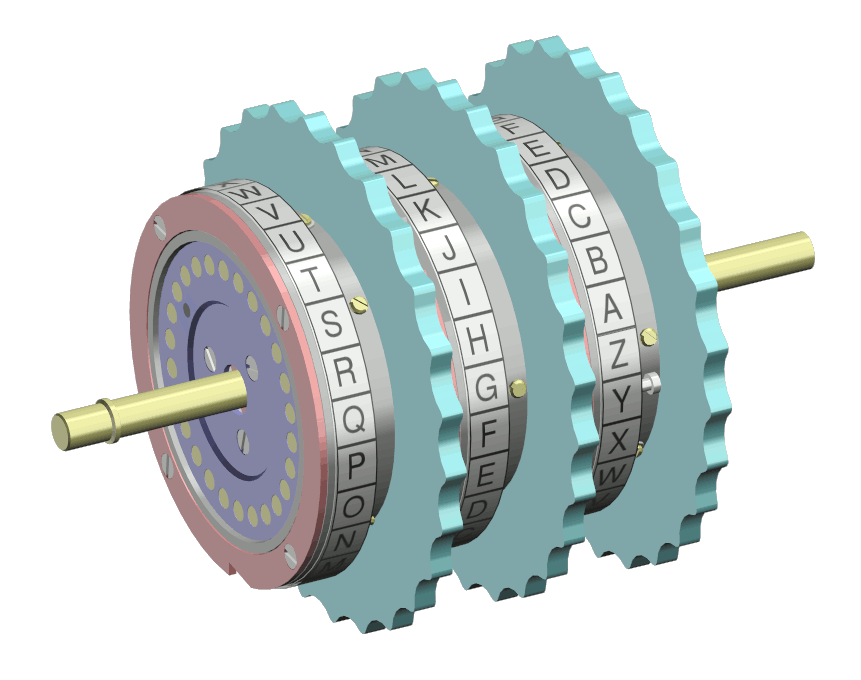
\includegraphics[width=.6\linewidth, keepaspectratio]{Enigma/Enigma-rotor-set}
	\caption{Enigma-Walzen\autocite{enigmarotorset2004}}
	\label{fig:enigma_rotors}
\end{figure}

Die Walzenstellung sagt aus, in welcher Ausgangsposition sich die Walzen befinden.
Diese kann durch ein Sichtfenster vom Bediener abgelesen werden.
Eine weitere Einstellmöglichkeit der Walzen ist die sogenannte Ringstellung.
Sie verändert die Relation der sichtbaren Buchstaben zu der internen Verdrahtung und bewegt die Übertragskerbe, %(siehe~\cref{fig:enigma-rotor-contact})
die festlegt, wann sich die Walze links von der aktuellen bewegt.
%Da die Ringstellung bei dem Entschlüsselungsverfahren der Turing-Bombe keine weitere Rolle spielt, wird hier nicht weiter darauf eingegangen.

%\begin{figure}[htbp]
%	\centering
%	\begin{tikzpicture}
%		\node at (0,0) {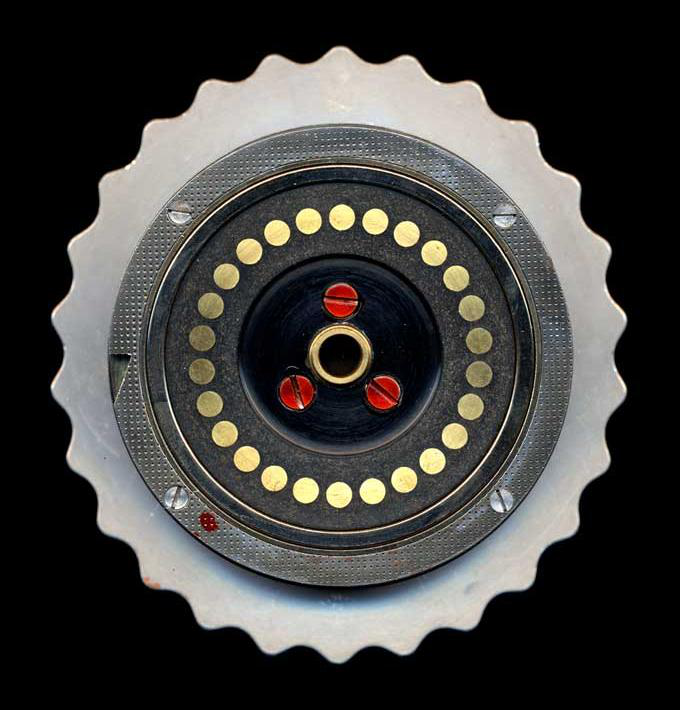
\includegraphics[width=.3\linewidth]{Enigma-rotor-flat-contacts.png}};
%		\draw[red, very thick, ->] (-3,-0.5) -- (-1.5,-0.1);
%		\node[red, anchor=west] at (-5,-0.8) {Übertragskerbe};
%	\end{tikzpicture}
%	\caption{Walzen Frontansicht mit Übertragskerbe}
%	\label{fig:enigma-rotor-contact}
%\end{figure}

\section{Umkehrwalze}\label{subsec:umkehrwalze}
Der originalen Patentschrift\autocite{scherbiuschiffriermaschine1925} von 1918 ist zu entnehmen, dass erste Enigma-Maschinen nicht involutorisch wirkten.
%Das bedeutet ganz allgemein, dass $E_K \ne D_K$ ist.
%$E_K$ ist die Chiffrierfunktion in Abhängigkeit eines Schlüssels – hier die Konfiguration der Enigma-Maschine.
%$D_K$ stellt die Dechiffrierfunktion dar.
%Es wird also zur Dechiffrierung eine andere Funktion, als zur Chiffrierung benötigt.
Konkret bedeutet das für sehr frühe Enigma-Maschinen, dass diese zur Dechiffrierung einer Nachricht, die zuvor von einer Enigma-Maschine chiffriert wurde, einen speziellen Modus benötigen.
Um die chiffrierte Nachricht zu dechiffrieren, muss ein Hebel umgelegt werden und die Walzen müssen in Ausgangsstellung gebracht werden.
Nun wird Strom nicht von rechts nach links, sondern von links nach rechts durch die Walzen geleitet.

Da das daraus resultierende Gesamtgewicht von rund 50\si{\kg} unakzeptabel für den Feldeinsatz war und der zusätzlich benötigte Mechanismus fehleranfällig erschien, wurde die Umkehrwalze oder auch der Reflektor von der Wehrmacht adaptiert.
Die Umkehrwalze sorgt dafür, dass 
%$E_K = D_K$ ist, sprich 
mit der gleichen Einstellung und \glqq Modus\grqq{} ein beliebiger Text sowohl chiffriert als auch dechiffriert werden kann.
Wie in~\cref{fig:enigma_reflector} zu erkennen, besitzt die Umkehrwalze nicht 52, sondern nur 26 Kontakte.
Sie \glqq wirft\grqq{} das Signal zurück und schickt dieses ein weiteres Mal, in entgegengesetzter Richtung durch die Walzen.
Es werden Buchstabenpaare gebildet, welche die Umkehrwalze kommutativ wirken lassen und die Enigma-Maschine involutorisch machen.
Somit wurde sich die Komplikation und das Gewicht des Dechiffrierungs-Modus gespart.

\begin{figure}
	\centering
	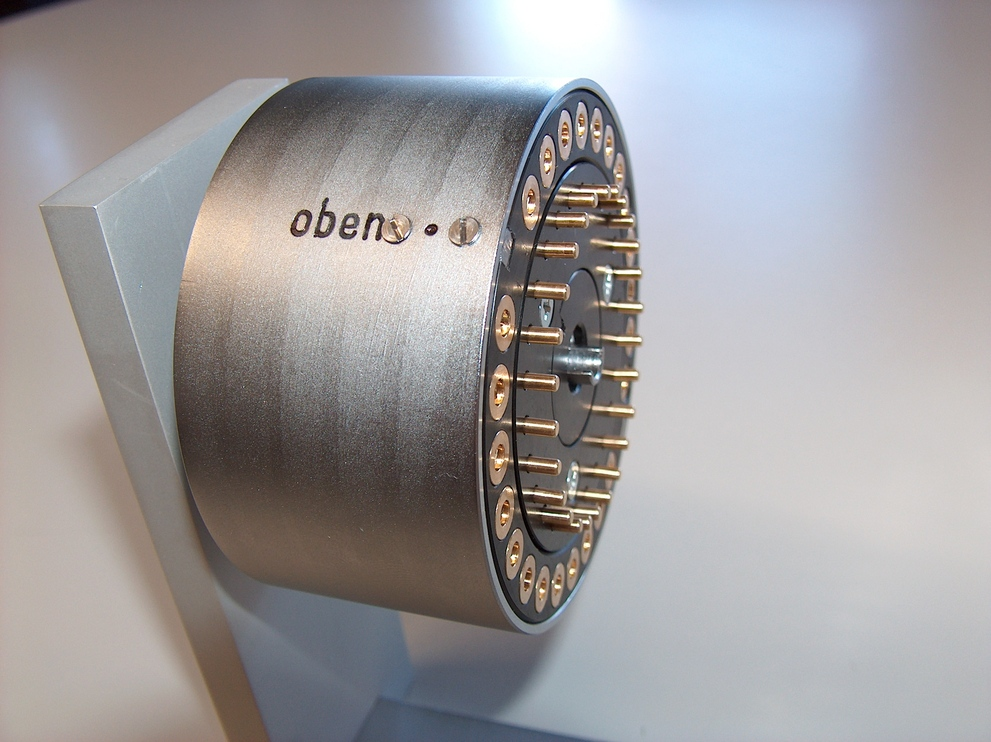
\includegraphics[width=.6\linewidth]{Enigma/UKW-D}
	\caption{Umkehrwalze-D Replika\autocite{enigmareflektor}}
	\label{fig:enigma_reflector}
\end{figure}

Doch leider ist dieser geniale Einfall die wohl größte Sicherheitslücke der Enigma.
Aufgrund der Buchstabenpaare wird niemals ein Buchstabe auf sich selber abgebildet.
Das Ergebnis ist eine sogenannte fixpunktfreie Permutation.
Kein Element behält somit seine Anfangsposition.
Da $\mathcal{A}\coloneqq\{\mathrm{A}, \mathrm{B}, \mathrm{C}, \ldots, \mathrm{Z}\},\; \forall x \in \mathcal{A}:\; E_K(x) \ne x$ bleiben nur noch wenige Positionen übrig, an welchen sich ein bekannter Funkspruch-Abschnitt (Known-plaintext) befinden kann.

%\newpage

\section{Steckerbrett}\label{subsec:steckerbrett}

Da ein Schlüsselraum von \num{686518560} Möglichkeiten\footnote{Diese Berechnung berücksichtigt die Anomalie des Fortschaltmechanismus.\autocite{wiki:enigma}} der Wehrmacht nicht genügte, wurde der Enigma-Maschine das Steckerbrett hinzugefügt.
Das Steckerbrett wirkt kommutativ und substituiert zwei Buchstaben. 
Es wird jeweils vor und nach dem Walzensatz traversiert. 
Die Anzahl von \num{150738274937250}\autocite{wiki:enigma} zusätzlichen Mög\-lich\-kei\-ten durch das Steckerbrett erscheint gewaltig, jedoch werden all diese Mög\-lich\-kei\-ten von der Turing-Welchman-Bombe überwunden und spielen für die Sicherheit der Maschine de facto keine Rolle.

\begin{figure}
	\centering
	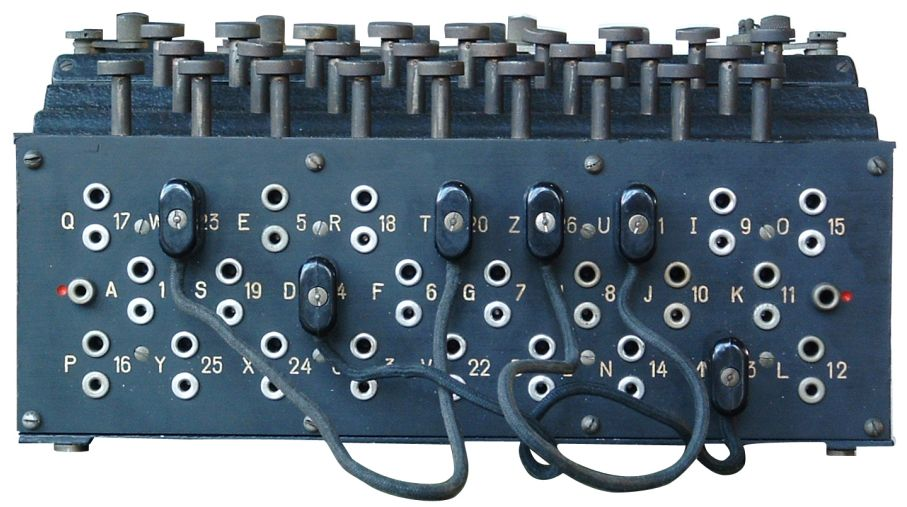
\includegraphics[width=.6\linewidth]{Enigma/enigma-steckerbrett}
	\caption{Enigma-Steckerbrett\autocite{wiki:enigmasteckerbrett}}
	\label{fig:enigma_plugboard}
\end{figure}

Die Permutation der Buchstaben lässt sich durch folgende Formel beschrieben.

Es sei:
\begin{itemize}
	\item $x \in \mathbb{Z}_{26}$: der zu permutierenden Buchstabe.
	\item $\tau_i(n)$: die Walzenstellung der Walze $i$ beim Tastendruck $n$.
	\item $W_i$: die feste Permutation der Walze $i$, das heißt $W_i: \mathbb{Z}_{26} \longmapsto \mathbb{Z}_{26}$.
	\item $W_i^{-1}$: die inverse Permutation der Walze $i$.
	\item $S$: die feste Permutation des Steckerbretts.
	\item $U$: die feste Permutation der Umkehrwalze.
\end{itemize}

So ergibt sich die folgende Funktion:

\[
	W_i^{\mathrm{rot}}(x) \coloneqq \left(W_i\left((x + \tau_i(n)) \mod 26\right) - \tau_i(n)\right) \mod 26
\]

Das gilt auch für die Inverse:

\[
	\left( W_i^{\mathrm{rot}}\right)^{-1} (x) \coloneqq \left(W_i^{-1}(\left(x + \tau_i(n)) \mod 26\right) - \tau_i(n)\right) \mod 26
\]

So ergibt sich:
\begin{equation}
	\label{eq:letter_permut}
	E_K(x) \coloneqq S\circ \left( W_1^{\mathrm{rot}}\right) ^{-1} \circ \left(W_2^{\mathrm{rot}}\right) ^{-1} \circ \left(W_3^{\mathrm{rot}}\right)^{-1} \circ U \circ W_3^{\mathrm{rot}} \circ W_2^{\mathrm{rot}} \circ W_1^{\mathrm{rot}} \circ S(x)
\end{equation}

\section{Übertragung der Nachrichten}\label{sec:uebertragung-der-nachrichten}
Bei der Enigma-Maschine wurde jeden Tag ein Tagesschlüssel eingestellt, welcher durch ein Code-Buch vorgegeben war.
Dieser Tagesschlüssel bestand darin, welche drei der acht Walzen der Schlüssler in welcher Reihenfolge einzusetzen hatte, welche Ringstellung und welche Steckerbrett-Verbindungen für den Tag gültig waren.
Von 13 möglichen Steckerbrett-Verbindungen wurden meistens 10 vorgegeben.
In~\cref{fig:enigma_code_book} ist ein Code-Buch-Auszug für eine Enigma-Maschine mit einer veränderlichen Umkehrwalze (UKW-D) zu sehen.

\begin{figure}
	\centering
	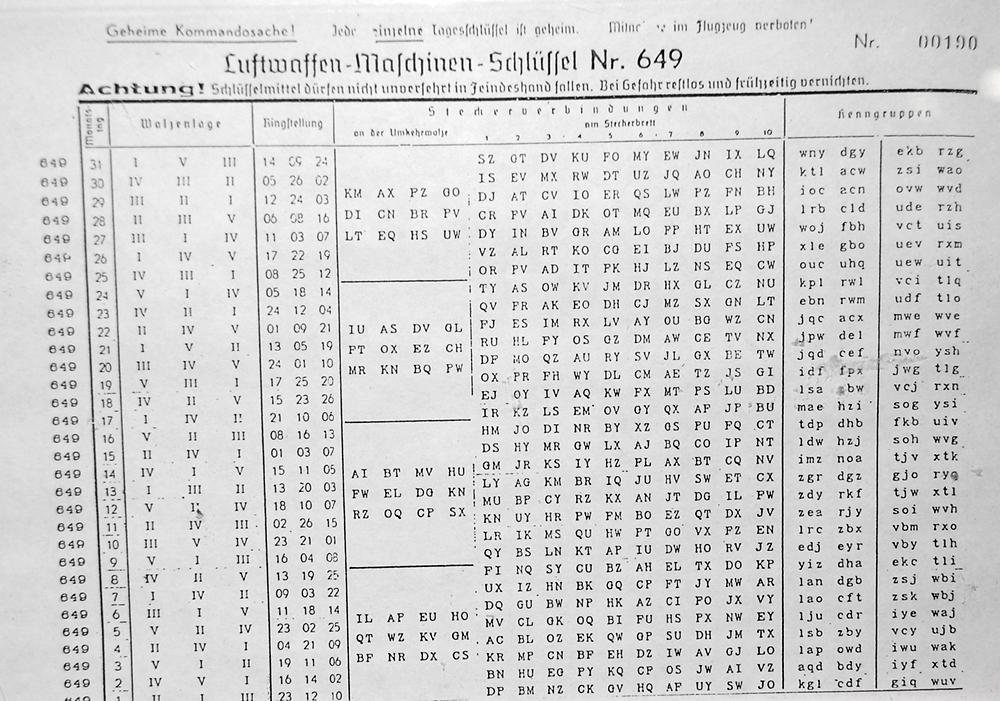
\includegraphics[width=.7\linewidth]{Enigma/Enigma-code-book}
	\caption{Code-Buch-Auszug\autocite{wiki:enigmacodebook}}
	\label{fig:enigma_code_book}
\end{figure}

Nach 1938 musste der Schlüssler sich eine eigene Grundstellung der Walzen überlegen, mit welchem er den sogenannten Spruchschlüssel verschlüsselte.
Nun überlegte sich der Schlüssler einen \glqq zufälligen\grqq{} Spruchschlüssel, mit dem der Text chiffriert wurde.\footnote{In Wahrheit wählten die Schlüssler oft den gleichen Schlüssel, der meist persönliche Informationen wie zum Beispiel den Namen der Freundin enthielt.}
Dieser Spruchschlüssel gibt die Walzenstellung für die folgende Nachricht an.
Der \glqq zufällige\grqq{} Spruchschlüssel wurde mit der Grundstellung verschlüsselt und ergab zusammen mit der Grundstellung und anderen Zusatzinformationen den \glqq Spruchkopf\grqq.
Dieser Spruchkopf wurde dann im Klartext an den Empfänger übertragen.  
Da jedoch die Ringstellung die Relationen der sichtbaren Buchstaben zu der internen Verdrahtung ändert, war die Information der Grundstellung und des Spruchschlüssels für die Alliierten nicht wirklich brisant.
Der Schlüssler gab den zu verschlüsselnden Text nach bestimmten Regeln ein\autocite{schluesselm1940}: Eigennamen wurden verdoppelt, Satzzeichen wie ein Punkt wurden durch ein X ersetzt, Uhrzeiten wurden ausgeschrieben und viele mehr.

Der Empfänger musste nun auf seiner Enigma-Maschine den Tagesschlüssel einstellen und die Walzen in die über den Spruchkopf mitgeteilte Grundstellung bringen.
Nun entschlüsselte er mit dieser Einstellung den Spruchschlüssel.
Wenn die Walzenstellung mitgeteilt durch den entschlüsselten Spruchschlüssel auf der Enigma-Maschine eingestellt wurde, konnte die eigentliche Nachricht dechiffriert werden.
In~Anhang~\ref{ch:msg-trans} ist der Vorgang einer Nachrichtenübertragung zu sehen.
Hierbei stellt $K_S$ den Spruchschlüssel und $K_T$ den Tageschlüssel dar.

\begin{samepage}
	Hierbei sei angemerkt, dass sich das Verfahren der Nachrichtenübertragung über die Kriegsjahre mehrfach änderte.
	So war die Grundstellung der Walzen vor 1938 noch Teil des Code-Buchs.
\end{samepage}

	
	\part{Die Turing-Welchman-Bombe}\label{ch:die-turing-bombe}

\chapter{Einführung}\label{sec:einfuerung_bombe}

Da frühe Verfahren zur Kryptoanalyse der Enigma-Maschine, wie zum Beispiel der \glqq Zyklometer\grqq{} oder die \glqq Bomba\grqq{}, durch die Einführung einer neuen Umkehrwalze (UKW-B), neuen Walzen und Änderung des Schlüsselverfahrens unbrauchbar gemacht wurden, musste ein neues Verfahren zur Kryptoanalyse der Enigma-Maschine von den Alliierten entwickelt werden. 
Der Durchbruch gelang, wie auch schon bei Marian Rejewski und seiner Bomba und Zyklometer, einem, beziehungsweise zwei Mathematikern.
Alan Turing und Gordon Welchman waren die Hauptverantwortlichen für die Entwicklung der \glqq Turing-Welchman-Bombe\grqq.
Dieses Verfahren basiert ähnlich wie der Zyklometer auf \glqq Zyklen\grqq.
Jedoch wurde hier nicht die Verdopplung des Spruchschlüssels im Spruchkopf ausgenutzt, sondern Zyklen zwischen einem an einer bestimmten Stelle im Geheimtext vermuteten Klartext (Crib) und dem Geheimtext bestimmt.
Die Turing-Welchman-Bombe testet immer eine Hypothese einer Steckerbrett-Verbindung und probierte mit drei von acht möglichen Walzen alle Walzenstellungen durch.
Auch wenn diese Hypothese sich als nicht korrekt erwies, findet die Turing-Welchman-Bombe bei korrekter Walzenlage durch Reductio ad absurdum trotzdem die gültigen Steckerbrett-Verbindungen.
Ziel war es, die abgefangene Nachricht und ultimativ den Tagesschlüssel zu knacken.
Aufgrund der Einfachheit wird im Folgenden der Begriff \glqq Bombe\grqq{} anstelle von \glqq Turing-Welchman-Bombe\grqq{} verwendet.
%\vspace{-13pt}
\begin{figure}
	\centering
	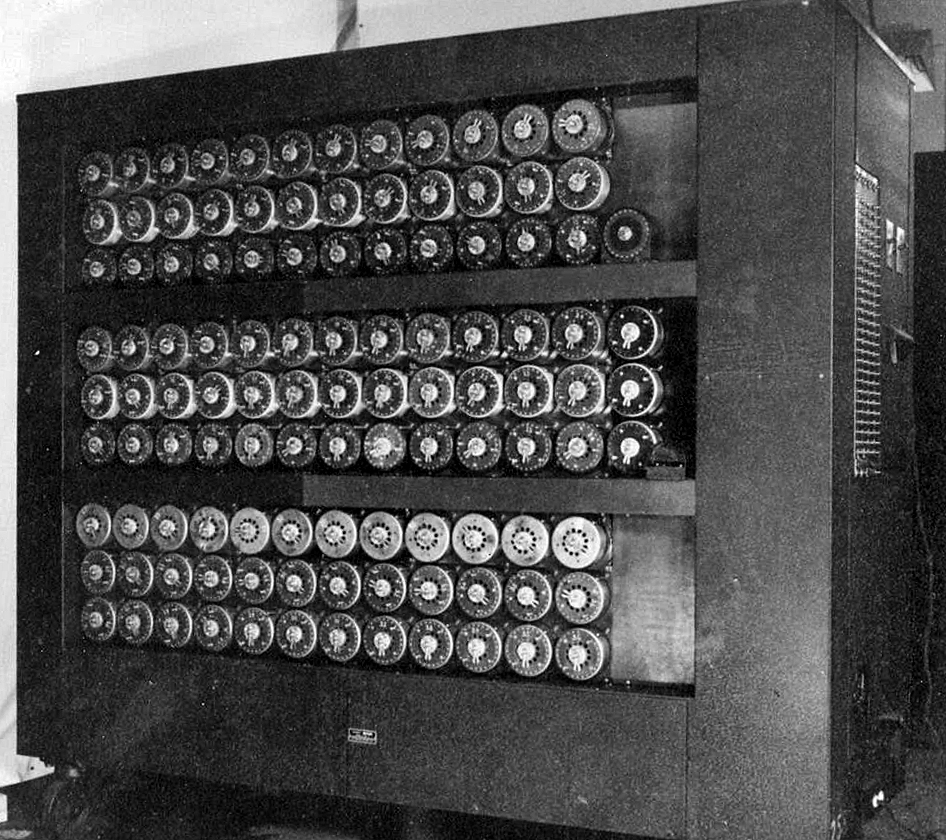
\includegraphics[width=.6\linewidth]{Turing Bomb/BletchleyParkBombe}
	\caption{Eine Turing-Welchman-Bombe in Bletchley Park\autocite{wiki:bombe_picture}}
	\label{fig:bombe}
\end{figure}

\chapter{Funktionsweise}\label{sec:funktionsweise_bombe}

\section{Vorbereitungen}\label{subsec:vorbereitungen}

\subsection{Crib}\label{subsubsec:crib}
Hier wird der Anglizismus \glqq Crib\grqq{} verwendet, da dieser Begriff keine richtige deutsche Übersetzung hat.

Ein Crib ist ein Klartextfragment, welches an einer bestimmten Stelle im Geheimtext vermutet wird. 
Die deutsche Wehrmacht verwendete in den gesendeten Nachrichten häufig Floskeln. 
Ein Beispiel hierfür ist: \glqq Das Oberkommando der Wehrmacht gibt bekannt\grqq.
Nun musste das Crib positioniert werden.
Wie in~\cref{subsec:umkehrwalze} erklärt, ist es nicht möglich, dass ein Buchstabe auf sich selbst abgebildet wird.
Wurde eine mögliche Position gefunden, konnten die Mitarbeiter von Bletchley Park anfangen, das sogenannte Menü zu bauen.
Die~\cref{fig:positioning_crib} zeigt solch eine Positionierung.

\begin{table}
	\centering
	\caption{Positionierung des Cribs}
	\label{fig:positioning_crib}
	\resizebox{\linewidth}{!}{
		\ttfamily\bfseries
		\begin{tabu}{c|c|c|c|c|c|c|c|c|c|c|c|c|c|c|c|c|c|c|c|c|c|c|c|c|c|c|c}
			B & H & N & C & X & S & E & Q & K & O & B & I & I & O & D & W & F & B & T & Z & G & C & Y & E & H & Q & Q & J \\
			O & B & E & R & K & O & M & M & A & N & D & O & D & E & R & \textcolor{red}{W} & E & H & R & M & A & \textcolor{red}{C} & H & T & & & &\\
			\rowfont{\color{DarkGreen}}
			\multicolumn{1}{c|}{} & O & B & E & R & K & O & M & M & A & N & D & O & D & E & R & W & E & H & R & M & A & C & H & T & & & \\
			\multicolumn{2}{c|}{} & O & B & E & R & K & O & M & M & A & N & D & \textcolor{red}{O} & \textcolor{red}{D} & E & R & W & E & H & R & M & A & C & \textcolor{red}{H} & T & & \\
			\rowfont{\color{DarkGreen}}
			\multicolumn{3}{c|}{} & O & B & E & R & K & O & M & M & A & N & D & O & D & E & R & W & E & H & R & M & A & C & H & T & \\
			\multicolumn{4}{c|}{} & O & B & \textcolor{red}{E} & R & \textcolor{red}{K} & \textcolor{red}{O} & M & M & A & N & \textcolor{red}{D} & O & D & E & R & W & E & H & R & M & A & C & H & T \\
		\end{tabu}
	}
\end{table}	

\smallskip
In Bletchley Park waren zudem viele Sprachexperten beschäftigt, die darauf spezialisiert waren, solche Cribs zu erstellen.
Dies erforderte sowohl sehr gute Kenntnisse über die deutsche Sprache, als auch sehr gute Kenntnisse über die in~\cref{sec:uebertragung-der-nachrichten}
beschriebenen Regeln zu Funkspruch-Verschlüsselung.
Zudem mussten Eigenheiten und die \glqq Schreibfäule\grqq{} der Funker beachtet werden.
Ein Crib wurde unter der Vermutung benutzt, dass während der kompletten Eingabezeit des Abschnittes nur die rechte Walze (schnelle) Walze rotiert hat.
Aus diesem Grund darf ein Crib nicht länger als 25 Buchstaben sein, da sonst gewiss ein Übertrag auf die mittlere Enigma-Walze stattfand.
Die Bombe vernachlässigt also den Übertragzeitpunkt der Enigma-Walzen, wodurch die Ringstellung keine weitere Rolle spielt.
Um das Risiko zu minimieren, dass ein Übertrag stattgefunden hat, wurden meist Cribs mit einer Länge von ungefähr 13 Buchstaben verwendet.
In unserem Fall wäre also das Crib \glqq OBERKOMMANDODERWEHRMACHT\grqq{} zu lang.
Da das Crib jedoch keinen linguistischen Sinn ergeben muss, könnte man dies einfach zu \glqq OBERKOMMANDODER\grqq{} kürzen.

Eine Strategie der Alliierten für die Erzeugung von Cribs war zum Beispiel das sogenannte \glqq Gardening\grqq.
Damit ist das bewusste provozieren von Funksprüchen, die einen bestimmten Klartext enthalten gemeint. % !
Eine Strategie war es, Seeminen in Flüsse, Häfen oder Seegebiete abzuwerfen.
Dafür musste ein Funker-Trupp in der Nähe des Ereignisses sein, welcher nicht verletzt werden durfte.
Ein mögliches Ziel war hier zum Beispiel ein Seegebiet in der Nähe eines U-Boots, da diese stets eine Enigma-Maschine an Bord hatten.
Nun beinhaltete der kurz darauf folgende Funkspruch mit einer hohen Sicherheit das Wort: \glqq Minen\grqq.

\subsection{Menü}\label{subsubsec:menu}
Nun werden Buchstaben-Tupel zwischen Crib und Geheimtext gebildet.
An einem Beispiel von \glqq WETTERVORHERSAGE\grqq{} und \glqq SNMKGGSTZZUGARLV\grqq{} wären solche Tupel: \texttt{W:S}, \texttt{E:N} et cetera.
Nun werden die Tupel mit passenden Buchstaben aneinander gesetzt. 
In dem obigen Beispiel wären die Tupel unter anderem: $\texttt{W:S} - \texttt{S:V} - \texttt{V:E}$.
Der daraus resultierende Graph wird \glqq Menü\grqq{} genannt.
Er gibt die Einstellungen der Bombe vor.
\nopagebreak
\begin{figure}
	\centering
	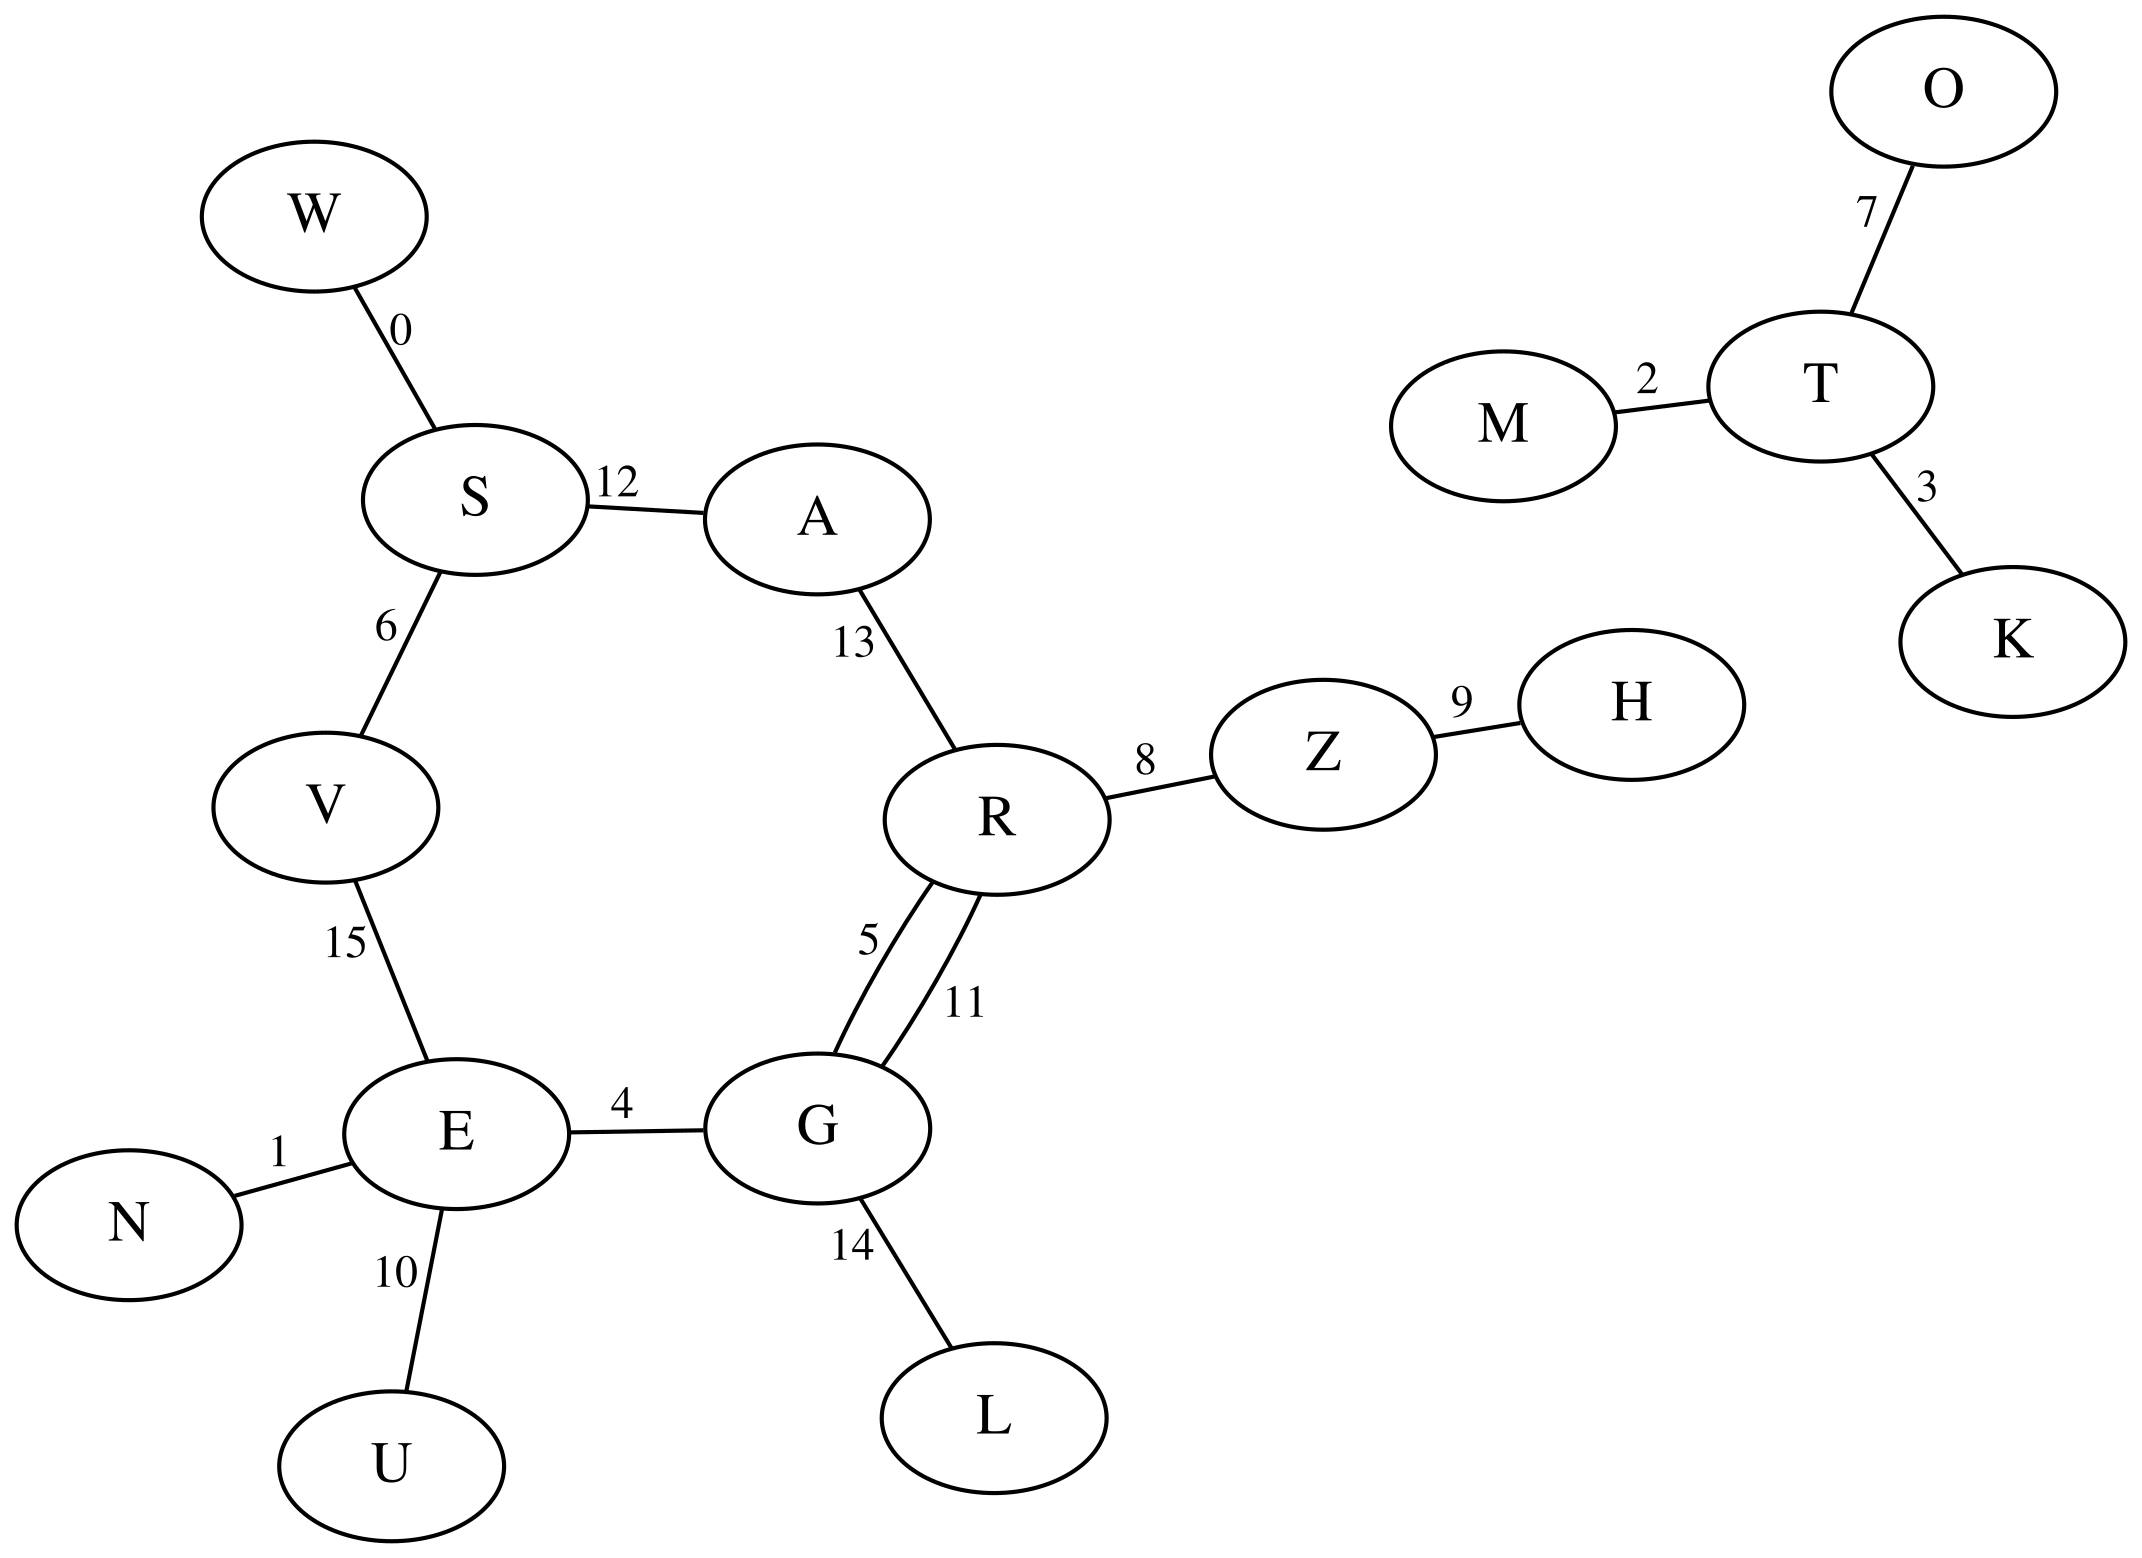
\includegraphics[width=.6\linewidth]{Turing Bomb/crib_cipher_cycle}
%	\includegraphics[width=.6\linewidth]{Turing Bomb/crib_cycle_cipher_graph}
	\caption{Crib-Geheimtext Menü}
	\label{fig:crib_cipher_cycle}
\end{figure}

Wenn sich wie in~\cref{fig:crib_cipher_cycle} ein Zyklus bildet, ist dies eine brauchbare Crib-Geheimtext-Kombination.
Alan Turing machte die Beobachtung, dass die Steckerbrett-Verbindungen der Enigma-Maschine keinen Einfluss auf den Verlauf des Menüs haben.
Dies ist durch die Eigenschaft des Steckerbrettes der Enigma-Maschine gegeben, welche eine monoalphabetische Substitution durchführt, die sich über den kompletten Chiffrierungs-Prozess nicht ändert.

Die Zahlen auf den Kanten geben hierbei die Position des Tupels innerhalb der gefundenen Crib-Geheimtext Kombination an.
Tupel wie 0, 1, 8, 9, 10 und 14 werden hier als \glqq Ausleger\grqq{} bezeichnet, da diese nicht aktiv zum Zyklus beitragen, aber trotzdem von Relevanz bei der Kryptoanalyse sind.
Aus Gründen, die später erläutert werden, sind Tupel-Kombinationen wie 5 und 11 äußerst effektiv für die Kryptoanalyse.
Tupel, die keinen Zyklus bilden, können ignoriert werden.
Somit sind die Tupel 2, 3 und 7 für den weiteren Verlauf der Kryptoanalyse irrelevant.

\section{Scrambler}\label{subsec:scrambler}
Wie auch die Enigma-Maschine hat auch die Bombe \glqq Walzen\grqq.
Jedoch haben diese nicht 52, sondern 104 Kontakte, da es erforderlich war, diese miteinander zu verbinden.
Die Walzen der Bombe werden oft Scrambler genannt.

\begin{figure}
	\centering
	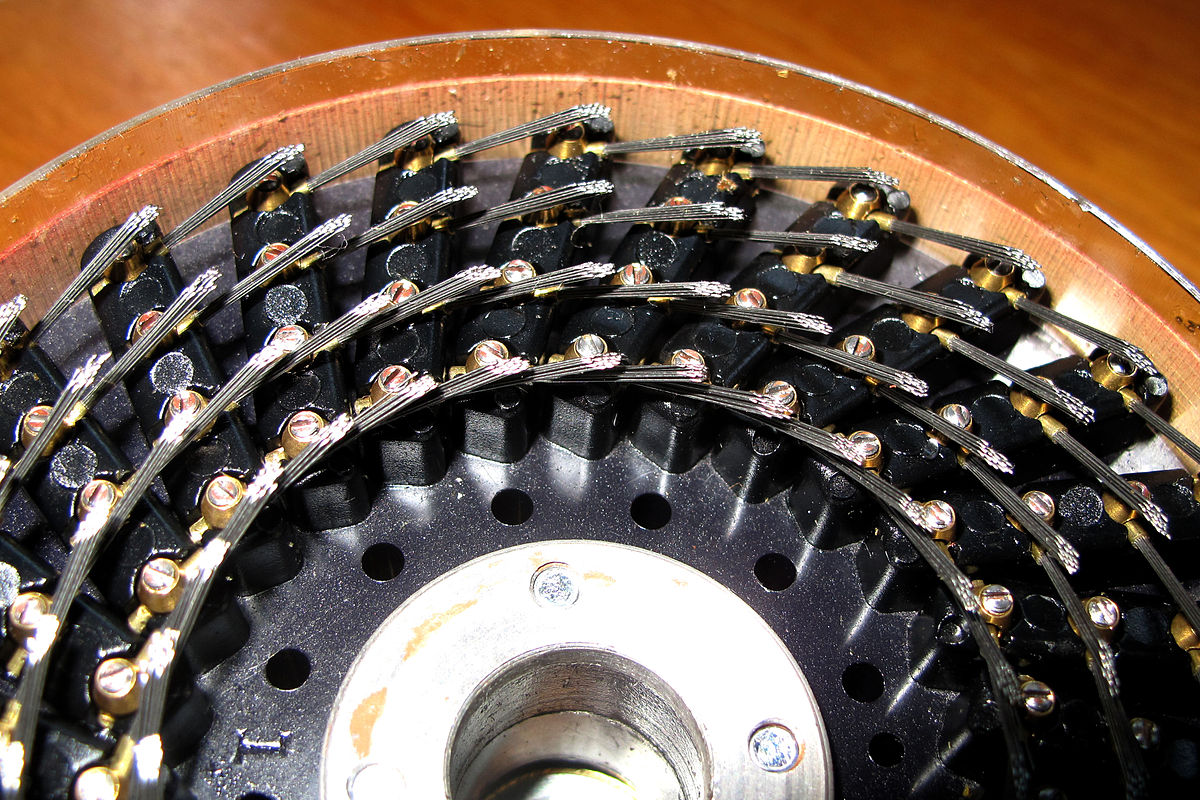
\includegraphics[width=.6\linewidth]{Turing Bomb/WireBrushesOnBombeDrum}
	\caption{Die Kontakte der Scrambler\autocite{wiki:bombescrambler}}
	\label{fig:scrambler}
\end{figure} 

Die meisten Bomben bestanden aus dreimal zwölf Scramblersätzen.
Zwölf Scramblersätze ergeben eine \glqq Chain\grqq.
Ein Scramblersatz bestand aus drei Scrambler und simulierte eine Enigma-Maschine.
Der Grund, warum zwölf \glqq Enigmas\grqq{} parallel verwendet werden, ist, da somit eine komplette Ausgangsstellung der Walzen für das jeweilige Crib in einem Arbeitsgang überprüft werden kann.
Der unterste Scrambler eines Scramblersatzes repräsentiert die rechte, schnelle Walze einer Enigma-Maschine.
Der mittlere und oberste Scrambler ist repräsentativ für die mittlere und linke Walze der Enigma-Maschine.
Da die Scrambler keine Übertragskerbe besitzen, bewegt sich der nächste Scrambler immer nach einer vollen Rotation des aktuellen Scramblers, unabhängig von der Startposition.

Wurde nun durch die Mitarbeiter von Bletchley Park ein passendes Menü bestimmt, konnten die Scrambler in ihre Ausgangsstellung gebracht werden. 
Hierfür muss in dem Zyklus eine \glqq Route\grqq{} bestimmt werden.
Für den Zyklus in~\cref{fig:crib_cipher_cycle} könnte die Route lauten: \texttt{W $\to$ S $\to$ A $\to$ R $\to$ G $\to$ E $\to$ V $\to$ S}.

Die Zahlen auf den Kanten werden als \glqq Offsets\grqq{} für die untersten Walzen benutzt.
In unserem Beispiel sind also die Ausgangsstellungen der Scrambler also \texttt{AAA}, \texttt{AAL} und so weiter.
Sollen jetzt auch noch Ausleger, oder andere Tupel-Kombinationen wie 5 und 11 eingebunden werden, so können diese einfach an passender Stelle eingefügt werden: \texttt{AAD, AAE, AAK}.
Die Gesamtlänge der Elemente des Zyklus darf nicht zwölf überschreiten.

\section{Terminal}\label{subsec:terminal}
Auf der Rückseite der Bombe befinden sich dreimal 26 Terminal-Kontakte.
Ein 26er-Terminal-Satz ist jeweils einer Chain zugeordnet.
Jeder Kontakt in einem Terminal-Satz repräsentiert jeweils einen Buchstaben im Alphabet.
Jeder der 26 Kontakte hat 26 kleinere Kontakte, die wieder das Alphabet repräsentieren.
Wird nun im \emph{A}-Terminal an den \emph{e}-Kontakt Spannung angelegt, so wird die Hypothese getestet, dass der Geheimtext mit der Steckerbrett-Verbindung $A \Leftrightarrow E$ verschlüsselt wurde.

\section{In und Outs}\label{subsec:in_und_out}
Auf der Rückseite befinden sich Kontakte, die mit \glqq In\grqq{} und \glqq Out\grqq{} gekennzeichnet sind.
Wieder drei mal zwölf In- und Out-Paare, jeweils für die Scramblersätze.
Nun werden die Terminals mit den In und Outs verbunden.
Da der gewählte Routen-Startpunkt bei \glqq W\grqq{} liegt, wird der erste Scramblersatz auf das Offset \texttt{AAA} eingestellt.
Darauf wird das Terminal \emph{W} mit dem ersten In-Kontakt verbunden.
Der nächste Routen-Punkt \glqq S\grqq{} wird durch einen \glqq Brücken-Konnektor\grqq{} dem ersten Out mit dem zweiten In und dem Terminal \emph{S} verbunden.

\section{Diagonalbrett}\label{subsec:diagonalboard}
Gordon Welchman fiel auf, dass bei frühen Bomben nicht die Kommutativität des Steckerbretts beachtet wurde.
Ist $A$ mit $B$ gesteckert, so muss auch $B$ mit $A$ gesteckert sein.
Das Diagonalbrett stellte diese kommutativen Verbindungen her.
Für die Bombe heißt dies, dass wenn im \emph{A}-Terminal an den \emph{b}-Kontakt Spannung angelegt wird,
so auch der \emph{a}-Kontakt im \emph{B}-Terminal aktiv wird.
Dies trug maßgeblich zur Effizienz der Bombe bei.
Der Kontakt gleich dem Terminal-Buchstaben wird \glqq Self-Steckered\grqq{} genannt und stellt keine Steckerbrett-Verbindung dar.

\begin{figure}
	\centering
%	\begin{tikzpicture}[scale=0.7, every node/.style={scale=0.8}]
%		\foreach \i in {0,..., 4}{
%			\foreach \j in {0,..., 4}{
%				\fill (\i*1.5, \j*1.5) circle (2pt); 
%			}
%			\draw (\i*1.5, \i*1.5) circle (4pt);
%
%		}
%		
%		\foreach \i in {1,...,4}{
%			\foreach \j in {1,...,4}{
%				\node[below] at (\i*1.5, \j*1.5) {\char\numexpr97+\i};			
%			}
%		}
%		
%		\foreach \i in {1,..., 4}{
%			\node[left] at (0, \i*1.5) {\char\numexpr65+\i};
%			\node[below] at (\i*1.5, 0) {\char\numexpr65+\i};
%		}
%		
%		\node[below left] at (0,0) {A};
%		
%		
%	\end{tikzpicture}
	\documentclass{standalone}
\usepackage{tikz}

\begin{document}
	\begin{tikzpicture}[scale=0.7, every node/.style={scale=0.8}]
		
		%Säulen
		\foreach \i in {0,2,4,6} {
			\foreach \j in {0,0.2,0.4,0.6} {
				\draw[thin] (\i+\j,1.5) -- (\i+\j,5+\j*2);
			}
			\node[below] at (\i+0.3, 1.5) {\emph{\char\numexpr65+\i/2}};
		}
		
		
		%Querverbindungen
		\foreach \j in {0.2,0.4,0.6} {
			\draw[thin](\j,5+\j*2) .. controls (\j*5,5+\j*1.5) .. (\j*10,5);
		}	
		
		\foreach \j in {0.4, 0.6} {
			\draw[thin](\j+2,5+\j*2) .. controls ({(\j + 2 + \j*10 + 0.2)/2},5+\j*1.6) .. (\j*10+0.2,5.4);
		}
		
		\draw[thin](4.6,6.2) .. controls (5.25,6.1) .. (6.4,5.8);
		
		%TODO at A terminal
		%		\draw[->] (-1,5.6) -- (0.2,5.4) node[left] at (-1,5.6) {\emph{b}-Kontakt im \emph{A}-Terminal};
	\end{tikzpicture}
\end{document}
	\caption{Diagonalbrett Verbindungen}
	\label{fig:diagonal_board_connections}
\end{figure}



\section{Commons}\label{subsec:commons}
Sollen nun auch noch Ausleger oder andere Graphen-Konstrukte miteinbezogen werden, reicht ein In- und Out-Kontakt nicht aus.
Hierfür gibt es dreimal sechs Common-Kontaktblöcke à fünf Kontakte.
Commons-Kontakte sind blockweise mit CO1, CO2 et cetera gekennzeichnet.
Sechs Blöcke sind einer Chain zugeordnet.
Die Kontakte eines Blocks sind miteinander verbunden.
Somit ist es möglich, den Out-Kontakt des Scramblersatzes, der dem \glqq E\grqq{} in unserem Zyklus entspricht, mit Terminal \emph{V} und \emph{N} und den jeweiligen Ins der Scramblersätze zu verbinden.
In~\cref{fig:bombe_rear} sind die Terminals, Commons und In und Outs mit den \glqq Brücken-Konnektoren\grqq{} zu sehen.
\nopagebreak
\begin{figure}
	\centering
	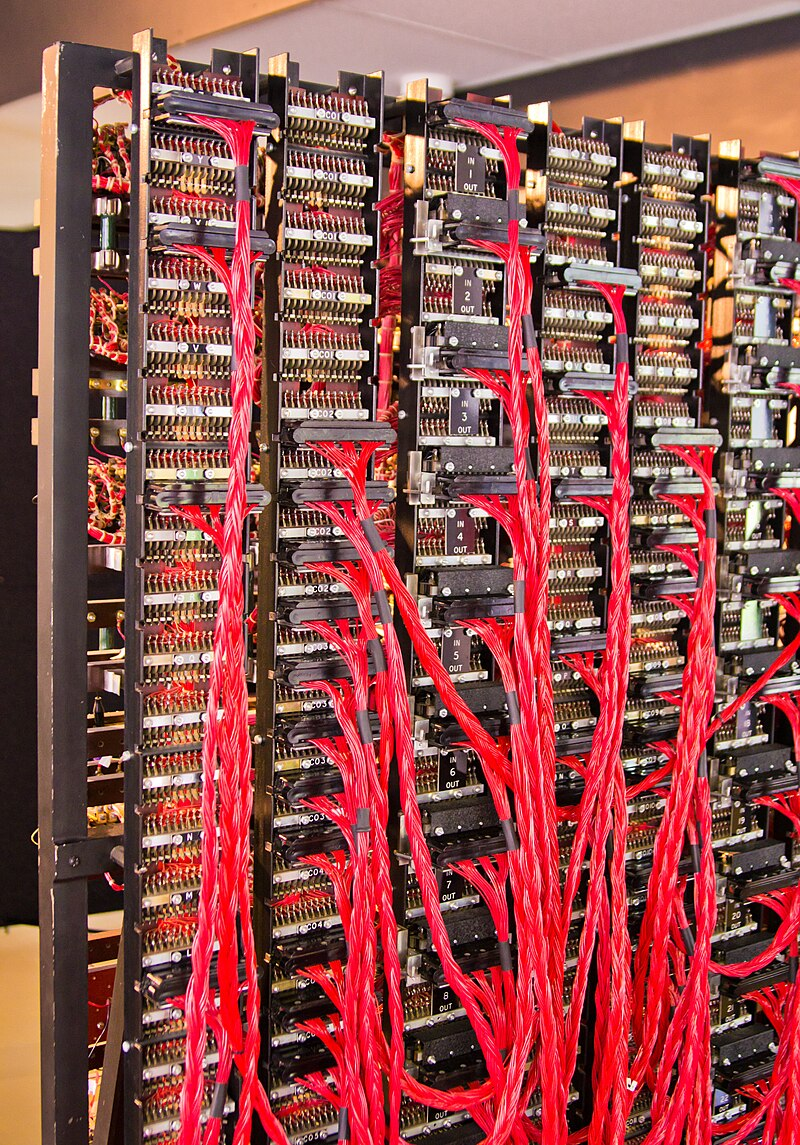
\includegraphics[width=.6\linewidth, clip, trim=2cm 25cm 5cm 2cm]{Turing Bomb/Bletchley_Park_Bombe_Rear}
	\caption{Rückansicht der Bombe\autocite{wiki:bomberear}}
	\label{fig:bombe_rear}
\end{figure}

\section{Test-Register}\label{subsec:test-register}
Um eine Steckerbrett-Verbindungs-Hypothese zu testen, muss ein Test-Register bestimmt werden. % !
Dies sollte ein Buchstabe im Menü sein, der sehr viele Verbindungen hat.
In dem Fall von~\cref{fig:crib_cipher_cycle} wäre der Buchstabe \glqq G\grqq{} geeignet.
Nun muss ein Test-Buchstabe bestimmt werden.
Fällt die Wahl zum Beispiel auf \emph{A}, so wird die Hypothese der Steckerbrett-Verbindung $A \Leftrightarrow G$ getestet.
Es wird vermutet, dass während des Chiffrierungs-Prozesses die Steckerbrett-Verbindung $A \Leftrightarrow G$ benutzt wurde.

\begin{figure}
	\centering
	\documentclass{standalone}
\usepackage{tikz}

\begin{document}
	\begin{tikzpicture}[scale=0.7, every node/.style={scale=0.8}]
		%Säulen
		\foreach \i in {0,2,4,6} {
			\foreach \j in {0,0.1,0.2,0.3} {
				\draw[thin] (\i+\j,1) -- (\i+\j,5+\j*2);
			}
			\node[below] at (\i+0.15, 1) {\emph{\char\numexpr65+\i/2}};
		}
		%		\draw[very thick] (2.2,1) -- (2.2,5.4);
		
		%		\draw[thin](0,9) .. controls (1,9.05) .. (2,9);
		
		%Querverbindungen
		\foreach \j in {0.1,0.2,0.3} {
			\draw[thin](\j,5+\j*2) .. controls (\j*10,5+\j*1.5) .. (\j*20,5);
		}	
		\draw[very thick] (0.1,1) -- (0.1,5.2) .. controls (1,5 + 0.1 * 1.5) .. (2,5) -- (2, 1);
		
		\foreach \j in {0.2, 0.3} {
			\draw[thin](\j+2,5+\j*2) .. controls ({(\j + 2 + \j*20 + 0.1)/2}, 5+\j*1.5) .. (\j*20 + 0.1, 5.2);
		}
		
		
		\draw[thin](4.3,5.6) .. controls (5.25,5.5) .. (6.2,5.4);
		
		\foreach \j in {0,0.1,0.2,0.3} {
			\draw[thin] (2+\j,2+\j) -- (4+\j,2+\j);
			\fill (2+\j,2+\j) circle (1pt);
			\fill (4+\j,2+\j) circle (1pt);
		}
		\fill (2.8, 1.9) rectangle (3.5, 2.4);
		\node[above] at (3.2, 2.4) {\texttt{1: AAA}};
		
		\foreach \j in {0,0.1,0.2,0.3}{
			\draw[thin] (\j, 3+\j) -- (4+\j, 3+\j);
			\fill (\j,3+\j) circle (1pt);
			\fill (4+\j,3+\j) circle (1pt);
		}
		
		\fill (0.8, 2.9) rectangle (1.5, 3.4);
		
		\node[above] at (1.2, 3.4) {\texttt{2: AAB}};
	\end{tikzpicture}
\end{document}
	\caption{Diagonalbrett Verbindungen mit Scrambler Verbindungen}
	\label{fig:diagonal_board_connections_w_scrambler}
\end{figure}

In~\cref{fig:diagonal_board_connections_w_scrambler} wird die Hypothese der Steckerbrett-Verbindung $A \Leftrightarrow B$ getestet.
Unser Test-Register ist \emph{A}.
Es wurde ein Scramblersatz mit der Grundstellung \texttt{AAA} konfiguriert und Terminal \emph{B} mit dem ersten In und Terminal \emph{C} mit dem ersten Out verbunden.
Ein weiterer Scramblersatz wurde auf die Grundstellung \texttt{AAB} konfiguriert und dem zweiten In mit dem ersten Out, welcher durch den Brücken-Konnektor auch mit Terminal \emph{C} verbunden ist, verbunden.
Außerdem wurde das zweiten Out mit Terminal \emph{A} verbunden.
Die Tupel in~\cref{fig:diagonal_board_connections_w_scrambler} sind \texttt{B:C} an erster und \texttt{C:A} an zweiter Stelle. 
Da das Steckerbrett keinen Einfluss auf den Verlauf des Zyklus hat, spielt es keine Rolle, welche Hypothese getestet wird.
%Der Zyklus-Verlauf für~\cref{fig:diagonal_board_connections_w_scrambler} ist B $\rightarrow$ C $\rightarrow$ A\textellipsis.
Nun wird \emph{a} durch den Scramblersatz permutiert.
Ergibt sich durch die Permutation von \emph{a} ein anderer Buchstabe als \emph{c}, müsste die Steckerbrett-Verbindung signalisiert durch den aktiven Kontakt während der Chiffrierung benutzt worden sein.

Die Bombe hält in zwei Fällen:
\begin{enumerate}
	\item In dem Test-Register ist nach den Permutationen ein Kontakt aktiv – die Hypothese hat sich bewahrheitet.
	\item In dem Test-Register sind nach den Permutationen 25 Kontakte aktiv – die Hypothese ist falsch, aber die nicht aktiven Kontakte in den Terminals geben die \glqq richtige\grqq{} Steckerbrett-Verbindung an. (Reductio ad absurdum)
\end{enumerate}

Die anderen Fälle werden von der Bombe ignoriert.
Angenommen unser erster Scramblersatz permutiert das \emph{a} im \emph{B}-Terminal zu einem \emph{c} und unser zweiter Scramblersatz permutiert dieses \emph{c} zu einem \emph{d} im \emph{A}-Terminal, so erzeugt dies ein Widerspruch.
Es wurde die Hypothese der Steckerbrett-Verbindung $A \Leftrightarrow B$ aufgestellt, aber damit der dritte Buchstabe im Zyklus bei der aktuellen Walzenlage einem \emph{a} entsprechen kann, muss zusätzlich $A \Leftrightarrow D$ herrschen.
Dies ist eine widersprüchliche Aussage, da Buchstaben nur mit einem anderen verbunden sein können –- die Walzen rotieren.

Die Tupel-Kombinationen 5 und 11 in~\cref{fig:crib_cipher_cycle} sind besonders effektiv, da sich die Anzahl der aktiven Verbindungen rasch \glqq aufschaukelt\grqq.



	
	\part{Implementierung der Turing-Welchman-Bombe}\label{ch:impl_bombe}
%\section{Enigma-Maschine}\label{sec:impl_enigma}
%Um die Bombe in Software Nachzubilden, muss zuerst eine Enigma-Maschine nachgebildet werden.
%\subsection{Rotoren}\label{subsec:impl_enigma_rotor}
%Die Verdrahtung der Rotoren wurden als Vektor realisiert.
%Der zu permutierende Buchstabe wird hierfür als Index in den Vektor genutzt.


\chapter{Menü Algorithmus}\label{sec:cycle-finding-algorithm}
Um eine Turing-Welchman-Bombe in der Programmiersprache C nachzubilden, muss zuerst ein Algorithmus entworfen werden, welcher das Menü durch ein von dem Nutzer vorgegebenes Crib und 
%TODO
Geheimtext bildet.

Hierfür werden die einzelnen Buchstaben als Knoten mithilfe einer Struktur dargestellt, welche zum einen den Buchstaben und zum anderen einen Vektor mit den anliegenden Auslegern beinhaltet.
Die Buchstaben-Tupel wurden ebenfalls als Struktur dargestellt, welche zwei Knoten, die Position im Crib und einen Booleschen Wert beinhaltet, welcher aussagt, ob dieses Tupel zum Zyklus beiträgt.

\begin{mylisting}
	\inputminted{C}{Implementierung/menu_structs.c}
	\caption{Realisierung der Menü Strukturen}
	\label{lst:code_impl_menu}
\end{mylisting}

%\begin{figure}
%\lstinputlisting[style=mystyle, caption={Realisierung der Menü Strukturen}, label={lst:code_impl_menu}]{Implementierung/menu_structs.c}	
%\end{figure}

Die Tupel werden nun in einer \glqq Nachschlagetabelle\grqq{} abgelegt.
Diese Tabelle hat 26 Stellen, repräsentativ für das Alphabet.
Ein jeweiliges Tupel wird sowohl unter dem ersten als auch unter dem zweiten Buchstaben abgelegt. 
Tupel wie \texttt{W:S} werden also unter \texttt{W} und unter \texttt{S} abgelegt.
Ein Tiefensuche-Algorithmus, der modifiziert wurde, um weniger \glqq gierig\grqq{} zu agieren, schlägt die Tupel in der Tabelle nach und markiert die besuchten Tupel.
%Bei dem Rücksetzverfahren der Tiefensuche wird die Markierung der Tupel, die nicht zum Zyklus beitragen entfernt.
Das Ergebnis ist eine gemessene, lineare Laufzeit.
\begin{marginfigure}
	\centering
	%	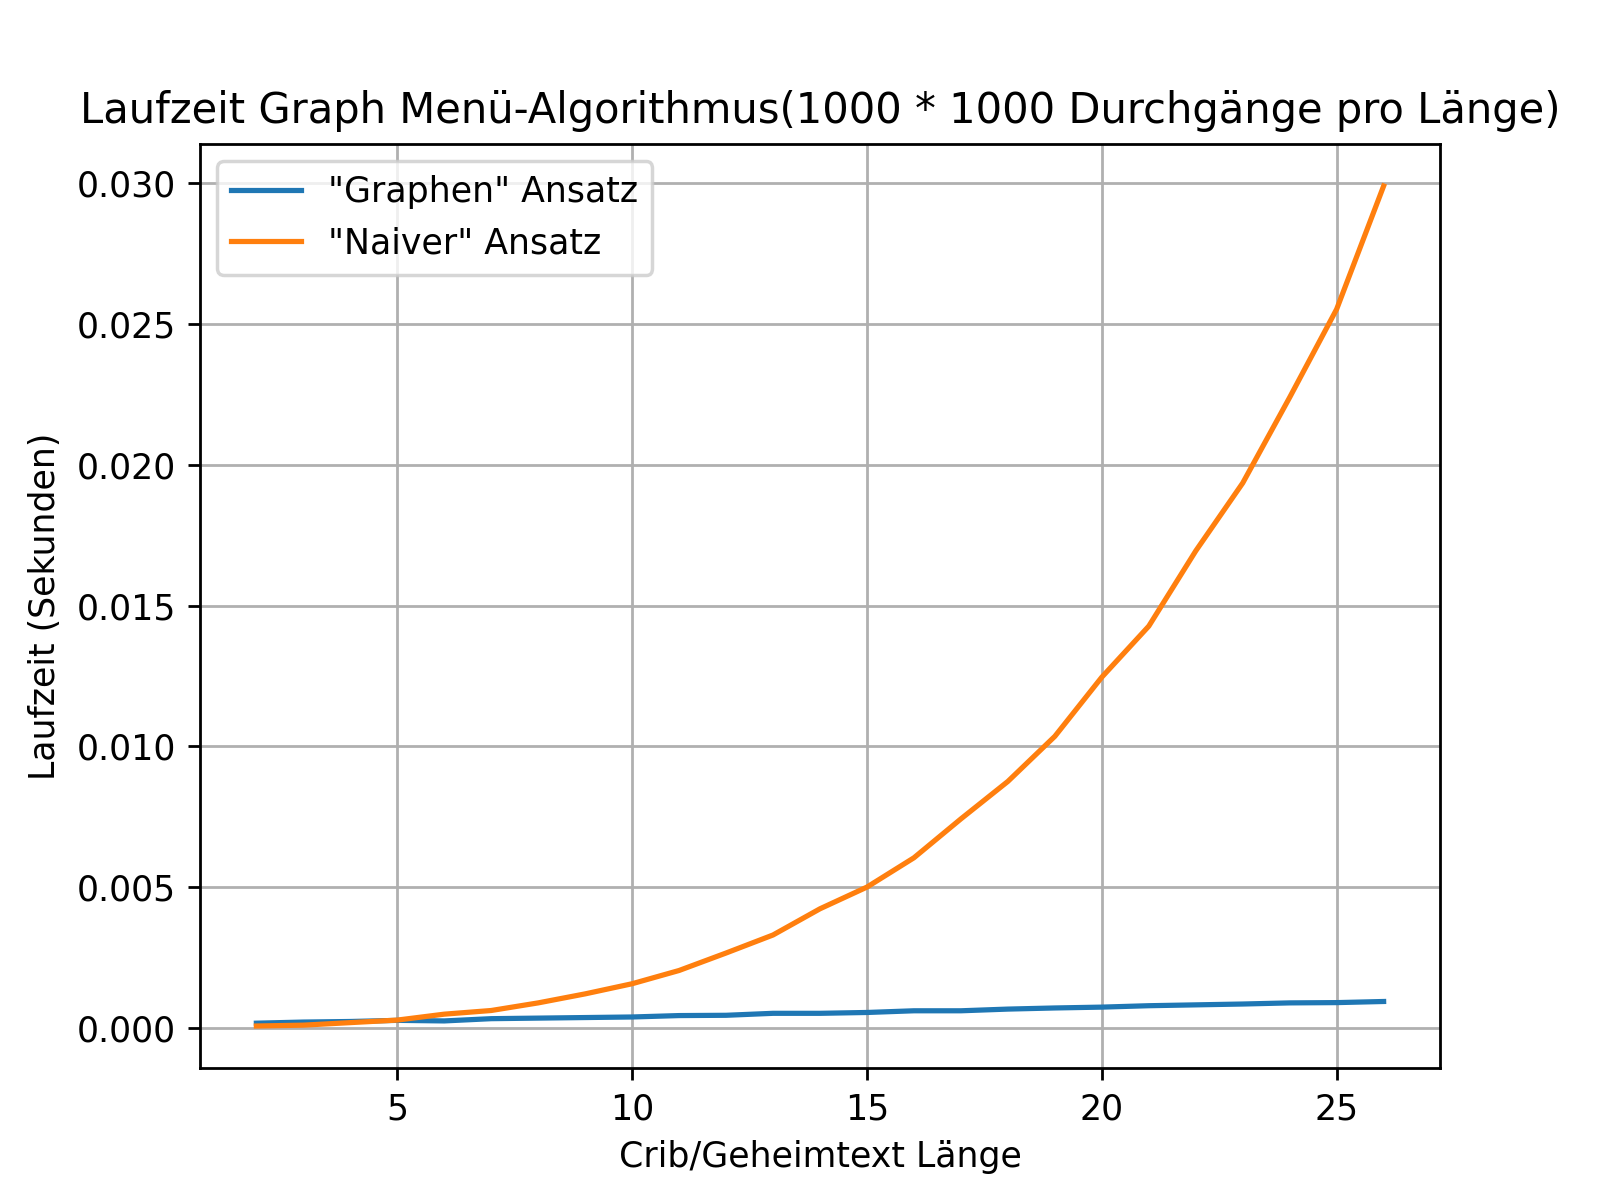
\includegraphics[width=.7\linewidth]{Turing Bomb/Crib-Cipher Loop/Runtime Graph Graph vs Force}
	\begin{tikzpicture}[scale=0.8]
		\begin{axis}[
			grid=major,
			xlabel={Inputvektor Länge},
			ylabel={Laufzeit (Sekunden)},
			axis lines=left,
			enlarge x limits={true},
			enlarge y limits={true},
			legend style={
				at={(0.4,1)},
				anchor=north,
				font=\small
			}
			]
			\addplot[thick, mark=none, gold] table[y=y1, x expr=\coordindex] {Turing Bomb/Crib-Cipher Loop/data.dat};
			\addlegendentry{"Graphen"-Algorithmus}
			\addplot[thick, mark=none] table[y=y2, x expr=\coordindex] {Turing Bomb/Crib-Cipher Loop/data.dat};
			\addlegendentry{"Naiver"-Algorithmus}
		\end{axis}	
	\end{tikzpicture}
	\caption{Der Laufzeit-Graph Menü-Algorithmus, getestet mit 1000 zufälligen Texten à 1000 Durchgänge.}
\end{marginfigure}
%\footnote{Es wurden Crib-Längen bis 26 betrachtet, um zu garantieren, dass die lineare Laufzeit bei einer maximalen Länge von 13 Buchstaben gegeben ist.
%Der Laufzeit-Graph ist im Anhang enthalten:~\cref{fig:app_menu_runtime}.}

Das Menü wird als Vektor von \texttt{CribCipherTuple} in einer Struktur mit der Länge abgelegt.
Da es erforderlich ist, eine eindeutige \glqq Route\grqq{} durch das Menü anzugeben, werden Tupel-Kombinationen bei den betroffenen Knoten als Ausleger angegeben. 
Die Bombe kann somit im Falle der \glqq Scramblersatz-Knappheit\grqq{} entscheiden, ob sie diesen (nicht notwendigen) Bestandteil des Menüs aufnehmen möchte.

\chapter{Modellierung der Turing-Welchman-Bombe}\label{sec:model}
\section{Scrambler}\label{subsec:impl_scrambler}
Wie in~\cref{subsec:vorbereitungen} erklärt, vernachlässigt die Bombe den Übertragzeitpunkt der Walzen.
Die Software-Implementation berücksichtigt ebenfalls die Übertragskerbe der Rotoren nicht.
%TODO Enigma Software gegeben erwähnen?
Die Verdrahtung der Scrambler wird als Vektor abgebildet, welcher wie in~\cref{fig:rot1_wiring} die Permutation für jeden Buchstaben speichert.
Die Buchstaben werden jedoch nicht in der typischen ASCII-Kodierung gespeichert, sondern auf den Wertebereich 0--25 abgebildet.
%TODO check
Mit dem Resultat kann somit direkt der Vektor des nächsten Scramblers indiziert werden.
Es muss zudem die Walzenlage mitgeführt werden, welche mit dem zu permutierenden Buchstaben addiert wird, um den Vektor-Index zu bilden.
Der Wertebereich wird durch eine Modulo-Operation zwischen 0 und 25 gehalten.

\section{Terminal}\label{subsec:impl_terminal}
Die Kontakte der Terminals werden als Struktur dargestellt.
Es beinhaltet einen 32-Bit-Integer, welcher als Bitvektor mit 26 seiner Stellen die aktiven Kontakte repräsentiert.
Die Anzahl der aktiven Kontakte wird ebenfalls als Integer mitgeführt.
Da es in Bezug auf die Laufzeit medioker ist, alle 26 Stellen des Bitvektors traversieren zu müssen, um zu überprüfen, welche der 26 Kontakte aktiv sind, wurde ein normaler Vektor eingeführt, der die aktiven Kontakte \glqq dicht\grqq{} speichert.
%TODO Artikel vor Nummer
Zuletzt wird der Buchstabe/die Nummer des jeweiligen Kontakts in der Struktur gespeichert.

\begin{mylisting}
	\inputminted{C}{Implementierung/terminal.c}
	\caption{Realisierung der Terminals}
	\label{lst:code_impl_terminal}
\end{mylisting}

Permutiert ein Scrambler einen Buchstaben, wird mithilfe des Bitvektors überprüft, ob dieser Kontakt bereits aktiv ist.

Hierbei gibt es zwei Szenarien:
\begin{enumerate}
	\item Der Kontakt ist inaktiv: In dem Bitvektor wird die repräsentative Stelle aktiviert, der Buchstabe wird in dem normalen Integer-Vektor abgelegt und die Anzahl der aktiven Verbindungen inkrementiert.
	
	\item Der Kontakt ist aktiv: Dieser Buchstabe wird ignoriert. 
\end{enumerate}

Die Terminal-Struktur beinhaltet einen Vektor mit 26 Kontakte und einen Zeiger auf den Kontakt des Test-Registers.
Bei dem Test-Register wird hierbei nicht von einem \glqq normalen\grqq{} Kontakt unterschieden.

\section{In und Outs}\label{subsec:impl_in_und_outs}
Die In- und Out-Kontakte werden mit dem dazugehörigen Scramblersätzen als Knoten dargestellt.
Sämtliche Verbindungen durch Kabel und Brücken-Konnektoren des analogen Originals werden hier durch Zeiger auf Kontakte ersetzt, so auch die In- und Out-Kontakte.

\section{Commons}\label{subsec:impl_commons}
Aufgrund der Einfachheit wurden die Commons in dieser Software-Imple\-men\-tation \glqq weg abstrahiert\grqq.
Diese wurden durch Zeiger auf den gleichen Kontakt ersetzt.
Die Anzahl der Kontakte pro Commons und die Gesamtzahl der verwendeten Commons wurde gezählt, sodass diese nicht die Anzahl des analogen Originals überschreiten.

\section{Diagonalbrett}\label{subsec:impl_diagonal_board}
Das Diagonalbrett als native Datenstruktur darzustellen, hat sich als ein eher schlechter Einfall herausgestellt.
Eine Möglichkeit, das Verhalten mit einer Datenstruktur zu imitieren, ist es, die einzelnen Kontakte der Terminals als Vektor mit Zeiger auf Booleschen Werten abzubilden.
Hierbei zeigt zum Beispiel der \emph{a}-Kontakt des \emph{B}-Terminals und der \emph{b}-Kontakt des \emph{A}-Terminals auf den gleichen Booleschen Wert.
Somit ist die Verbindung $A \Leftrightarrow B$ abgebildet.
Jedoch wäre es hier abermals nötig, den gesamten Vektor zu traversieren, um die aktiven Kontakte herauszufinden.
Die entsprechenden Kontakte müssten nun wieder einen normalen Vektor besitzen, in dem die aktiven Kontakte \glqq dicht\grqq{} stehen, damit die Scrambler effektiv arbeiten können.
Somit wäre es hier abermals notwendig, die Kontakte separat zu behandeln.

Aus diesem Grund wurde die Funktion des Diagonalbrettes in einer Funktion gekapselt:

\begin{mylisting}
	\inputminted{C}{Implementierung/diag_method.c}
	\caption{Realisierung des Diagonalbrettes}
	\label{code_impl_diag_board}
\end{mylisting}

%TODO TuringBombe Struct erklären?
Diese Funktion erhält drei Argumente: Einen Zeiger auf eine \texttt{TuringBombe} und zwei Integer, repräsentativ für die zwei Terminal-Buchstaben, die aktiviert werden sollen.

\chapter{Algorithmus der Implementation}\label{sec:algorithm_bombe}
Im Gegensatz zur \glqq echten\grqq{} Bombe, welche eine Steckerbrett-Hypothese für die jeweils 17576 Walzenstellungen einer Walzenlage testet, testet die Software-Nachbildung eine Hypothese für alle Walzenstellungen der 60 möglichen Walzenlagen.
Eine modifizierte Breitensuche traversiert die Knoten des aufgespannten Graphen der \glqq Scrambler-Knoten\grqq.
Da es aufgrund der Tupel-Kombinationen nicht genügt, einige Knoten nur einmal zu besuchen, und das Diagonalbrett es schwierig macht, die Datenstruktur der Knoten linear zu durchlaufen, wird erneut eine \glqq Nachschlagetabelle\grqq{} benötigt.
Die Nachschlagetabelle besitzt 26 Stellen, jeweils für die 26 Terminal-Kontakte.
Die Knoten, die durch den In-Kontakt mit einem jeweiligen Terminal verbunden sind, werden in dieser Tabelle abgelegt.
Zuerst werden alle Scrambler-Knoten, die durch den In-Kontakt mit dem Test-Register verbunden sind, in die Warteschlange eingereiht. 
Danach werden die Commons der jeweiligen Knoten eingereiht und als Letztes die Knoten, welche an jene Kontakte anliegen, die durch direkte Permutation der Scrambler oder durch das Diagonalbrett aktiviert wurden.
Wird durch die Permutation eines Scramblers in dem mit ihm verbundenen Out-Kontakt kein neuer Kontakt aktiv, so werden die Knoten, welche durch den In-Kontakt mit dem jeweiligen Kontakt verbunden sind, nicht eingereiht.
%wird dieser Knoten als \glqq besucht\grqq{} gekennzeichnet und nicht mehr in die Warteschlange eingereiht.
Ist die Warteschlange leer, ergo keine Permutationen mehr möglich, wird das Test-Register überprüft.
%sind alle Permutationen abgeschlossen und das Test-Register wird überprüft.
Ergeben die Permutationen keine gültige Konfiguration, werden alle Kontakte die durch Permutation oder Diagonalbrett aktiviert wurden, deaktiviert. 
%und Knoten als nicht besucht gekennzeichnet.
Die Software-Nachbildung hält nach den in~\cref{subsec:test-register} beschriebenen Regeln.
%In Pseudocode könnte man den Algorithmus der Bombe so darstellen:
%\begin{algorithm}[htbp]
%	\caption{Bombe Algorithmus}
%	\begin{algorithmic}
%			\Procedure{Bombe}{$p_0 \dots p_{n-1} :$ [Char], $c_0 \dots c_{n-1} :$ [Char]}
%			\ForAll{\textsl{rotors} $\in$ \textbf{permut(rotor order)}, \textsl{pos} $\in$ \textbf{[AAA $\dots$ ZZZ]}}
%			\State plugs: Char $\rightarrow \{ $Char$\}$
%			\State plugs$(p_0)\ \cup= \{\textbf{'A'}\}$
%			\While{\textsl{plugs} changing}
%			\ForAll{\textsl{i} $\in$ \textbf{[0\dots n--1]}}
%			\State plugs($c_i$) $\cup=$ $\bigcup_{p \in \text{plugs}(p_i)}$ encrypt(\textsl{rotors, p, pos}+\textsl{i})
%			\State plugs($p_i$) $\cup=$ $\bigcup_{p \in \text{plugs}(c_i)}$ encrypt(\textsl{rotors, p, pos}+\textsl{i})
%			\EndFor
%			\EndWhile
%			\If{$\forall$ \textsl{S} $\in$ \textbf{cod(plugs)}: \#S < \#Char}
%			\State report(\textsl{pos, plugs})
%			\EndIf
%			\EndFor
%			\EndProcedure
%		\end{algorithmic}
%	\label{alg:algorithm}
%\end{algorithm}

	
	\part{Geschwindigkeit der Software-Nachbildung im Kontext}\label{ch:speed}

\chapter{Koinzidenzindex}\label{sec:koinzidenzindex}
Hatte die Bombe gestoppt, machten sich die Mitarbeiter in Bletchley Park daran, den Stopp zu "bewerten". 
Genauer wird überprüft, ob die Enigma-Konfiguration, signalisiert durch den Stopp, zu einem sinnvollen Ergebnis führt.
%In Bletchley-Park wurde diese Bewertung durch einen oder mehrere Linguistikexperten durchgeführt.
Zunächst wird ein Maß benötigt, mit welchem sich teilweise/vollständig dechiffrierte Texte "bewerten" lässt.
Ein geeignetes Maß für die Annäherung eines Textes an authentisches Deutsch ist der Koinzidenzindex:

\begin{equation}
	\label{eq:koinzidenindex}
	IC = \frac{1}{N(N-1)}\sum_{i\in\mathcal{A}}f_i(f_i-1)
\end{equation}
	
	
Sei $f_i$ die Häufigkeit des Buchstabens in Abhängigkeit von $i$ und $N$ die Gesamtanzahl der Buchstaben.
%Wir Summieren also die Anzahl der Buchstabenpaare auf, und teilen diese durch die Anzahl der allgemein möglichen Buchstabenpaare.
Der Koinzidenzindex ist ein statistisches Maß zur Analyse der Häufigkeitsverteilung der Buchstaben.
Für einen Text, bestehend aus zufälligen Buchstaben, beträgt der $IC \approx 0.038$, wobei er für Deutsch $\approx 0.078$ beträgt.
Ermittelt die Nachbildung einen Stopp, so wird der gesamte Geheimtext dechiffriert und mit dem Koinzidenzindex bewertet.
Gemessen wird der "Abstand" zum Referenzwert 0.078.
Texte, bei denen der Abstand des Koninzidenzindexes am geringsten ausfällt, werden am höchsten bewertet.


\chapter{Geschwindigkeit im Kontext der "echten" Bombe}\label{sec:speed}
Um die Geschwindigkeit der Software-Implementierung in einen Kontext zu setzen, muss zuerst die Entschlüsselungsprozedur betrachtet werden.
In Bletchley Park waren zu Kriegsende mehr als 210 Bomben im Einsatz.
Der Bombe ist es möglich, eine Walzenlage innerhalb von etwa 20 Minuten abzuarbeiten.
Da über 210 Bomben zu Verfügung standen, war es möglich alle 60 Walzenlagen in dieser Zeit abzuarbeiten.
%Da das bewerten eine mühselige Handarbeit war, konnte die letztendliche Entschlüsselung des Tagesschlüssels 2-4 Stunden andauern.
Die Bestimmung des Menüs, Konfiguration der Bombe und die Bewertung der Walzenlagen in Bletchley Park war Handarbeit.
Deshalb variierte die Arbeitszeit bis zur Brechung des Schlüssels im Mittel zwischen 2-4 Stunden.
Die Bestimmung des Cribs beruhte einzig und allein auf der Expertise der Linguistischen Experten. 
Aus diesem Grund wurden manche Schlüssel gar nicht gebrochen.
Leider sind mögliche Heuristiken bei der Überprüfung der Stopps nicht überliefert.

\begin{table}
	\centering
	\caption{Geschätzte Anzahl der Stopps pro Walzenlage~\autocite{enwiki:bombe}}
	\label{tab:num-stops}
	\resizebox{\linewidth}{!}{
	\begin{tabular}{|c||c|c|c|c|c|c|c|c|c|}
		\hline
		                                    &              \multicolumn{9}{c|}{Buchstaben im Menü}               \\ 
		              Zyklen                &   8   &   9   &  10  &  11  &  12  &  13   &  14   &  15   &  16   \\
		\hhline{|=||=|=|=|=|=|=|=|=|=|}
						 3 					&  2.2  &  1.1  & 0.42 & 0.14 & 0.04 & $<0.01$ & $<0.01$ & $<0.01$ & $<0.01$ \\ \hline
		                 2                  &  58   &  28   &  11  & 3.8  & 1.2  & 0.30  & 0.06  & $<0.01$ & $<0.01$ \\ \hline
		                 1                  & 1500  &  720  & 280  & 100  &  31  &  7.7  &  1.6  & 0.28  & 0.04  \\ \hline
		                 0                  & 40000 & 19000 & 7300 & 2700 & 820  &  200  &  43   &  7.3  &  1.0  \\ \hline
	\end{tabular}
	}
\end{table}

\smallskip
Wie in~\cref{tab:num-stops} zu sehen, hängen die Anzahl der Stopps stark von der "Güte" des Menüs ab.
Die Software-Implementation benötigt für Erstellen eines Menüs der Länge zwölf, die Abarbeitung aller Walzenlagen und das "bewerten" der Stopps im Mittel
%TODO checking machine time
$150\si{\ms}$.

\[
\frac{3\si{\hour} \cdot 60 \cdot 60 \cdot 1000}{150\si{\ms}} \approx 72000
\]

Ein moderner Computer\footnote{Systemspezifikationen im Anhang enthalten:~\cref{tab:sys-spec}.} ist somit um Faktor 72000 schneller, als der kombinierte Kriegsaufwand der knapp 9000 Bletchley Park Mitarbeiter.
Es sei angemerkt, dass die Bewertung der Stopps durch Linguistische Experten hochwertiger ist, als der Koinzidenzindex.

	
	\backmatter
	\pagestyle{empty}
	\clearpage
	\phantomsection
	\addcontentsline{toc}{part}{Glossar}
	\chapter*{Glossar}\label{sec:glossar}
	\begin{itemize}
		\item Bletchley Park: Zentrale militärische Dienststelle, die sich im Zweiten Weltkrieg erfolgreich mit der Entzifferung des deutschen Nachrichtenverkehrs befasste.
		\item Crib: Klartextfragment, welches an einer bestimmten Stelle im Geheimtext vermutet wurde.
		\item $D_K$: Die Dechiffrierfunktion.
		\item $E_K$: Die Chiffrierfunktion.
		\item Gardening: Das Provozieren von Funksprüchen, welche einen bestimmten Klartext enthalten.
		\item Menü: Ein Graph aus Crib-Geheimtext Tupeln, der die Einstellungen der Bombe vorgibt.
		\item Involution: Eine selbstinverse Abbildung.
		\item Schlüssler: Person, die Nachrichten ver- oder entschlüsselt.
		\item Spruchkopf: Unverschlüsselter, erster Teil einer Nachricht, welcher die Uhrzeit, die Buchstabenanzahl, die Grundstellung und den verschlüsselten Spruchschlüssel beinhaltete.
		\item Spruchschlüssel:  Individueller Schlüssel für einen Funkspruch.
	\end{itemize}
	\clearpage
	
	\phantomsection
	\addcontentsline{toc}{part}{Quellen}
	\chapter*{Quellen}\label{ch:sources}
	\section{Einzelnachweise}\label{sec:einzelnachweise}
	\printbibliography[keyword=sources, heading=none, title={}]
	\section{Bildnachweise}\label{sec:bildnachweise}
	\printbibliography[keyword=pictures, heading=none, title={}]
	\nocite{*}
	\thispagestyle{plain}
	
	\appendix
	\part{Anhang}
	\chapter{Übertragung der Nachrichten}\label{ch:msg-trans}
\begin{fullwidth}
	\includegraphics[width=\linewidth]{Anhang/message_transmission}
\end{fullwidth}

\chapter{Systemspezifikationen}\label{ch:sys-spec}
\begin{table}[htbp]
	\centering
	\caption{Systemspezifikationen Referenzsystem}
	\label{tab:sys-spec}
	\begin{longtable}{|>{\raggedright\arraybackslash}p{4cm}|>{\raggedright\arraybackslash}p{5cm}|}
		\hline
		\textbf{Komponente} & \textbf{Spezifikation} \\
		\hline
		\endfirsthead
		\hline
		\textbf{Komponente} & \textbf{Spezifikation} \\
		\hline
		\endhead
		\hline
		\endfoot
		
		\textbf{Prozessor} &  AMD Ryzen 9 5900X \\
		\hline
		\textbf{Arbeitsspeicher (RAM)} & 32 GB DDR4, 3600 MT/s \\
		\hline
		\textbf{Grafikkarte} & NVIDIA GeForce RTX 3070, 8 GB GDDR6 \\
		\hline
		\textbf{Festplatte (SSD)} & 1 TB NVMe M.2 SSD \\
		\hline
		\textbf{Betriebssystem} & Windows 11 Pro, 64-bit \\
		\hline
		\textbf{Netzteil} & 850 W, 80 PLUS Gold zertifiziert \\
		\hline
		\textbf{Kühlung} & Wasserkühlung (420mm Radiator) für CPU \\
		\hline
	\end{longtable}
\end{table}
\end{document}
